\documentclass{article}
\usepackage{graphicx, color, amssymb, amsmath, bm, rotating, graphics,
epsfig, multicol, amsthm, bbm}
\usepackage{multicol}
\usepackage{textcomp}
\usepackage{fullpage}
\usepackage{booktabs}
\usepackage{caption}
\usepackage[authoryear]{natbib} %numbers instead of authoryear for [1] instead of [1980]
%Indicator function: use as \indicator{X=x}
\newcommand{\indicator}[1]{\mathbbm{1}{\left\{ {#1} \right\} }}
%Independent: use as X \ind Y | Z
\newcommand\ind{\protect\mathpalette{\protect\independenT}{\perp}}
\def\independenT#1#2{\mathrel{\rlap{$#1#2$}\mkern2mu{#1#2}}}
\newtheorem{alg}{Algorithm}
\newtheorem{thm}{Theorem}[subsection]
\newtheorem{prop}[thm]{Proposition}
\newtheorem{cor}[thm]{Corollary}
\DeclareMathOperator{\tr}{tr}
\DeclareMathOperator{\B}{B}
\DeclareMathOperator{\vech}{vech}
\DeclareMathOperator{\vect}{vec}


\newcommand{\matt}[1]{{\color{red} Matt: #1}}

\begin{document}


\title{Ancillarity-Sufficiency or not; Interweaving to Improve Markov Chain Monte Carlo (MCMC) Estimation of the Dynamic Linear Model (DLM)}
\author{Matt Simpson}
\maketitle

\begin{abstract}
In DLMs, MCMC sampling can often be very slow for accurately estimating the posterior density --- especially for longer time series. In particular, in some regions of the parameter space the standard data augmentation algorithm can mix very slowly. Using some of the insights from the data augmentation for multilevel models literature, we explore several alternative data augmentations for a general class of DLMs and we show that no ``practical'' centered parameterization (or sufficient augmentation in the terminology of \citet{yu2011center}) exists. In addition, we utilize these augmentations to construct several interweaving algorithms --- though we cannot construct an ancillary-sufficient interweaving algorithm (ASIS) since no sufficient augmentation exists, we find two ancillary augmentations and are able to construct a componentwise interweaving algorithm (CIS) that uses ASIS for each model parameter conditional on the rest. Using the local level DLM, we show how to construct several of these algorithms and conduct a simulation study in order to discern their properties. We find that several algorithms that outperform the usual ``state sampler'' for many values of the population parameters, though there is room for improvement.
\end{abstract}


\section{Introduction}\label{sec:Intro}

\matt{need more here}

\subsection{Data augmentations}
Ever since the seminal article by \citet{tanner1987calculation}, data augmentation has become a common strategy for constructing MCMC algorithms to sample from intractable probability distributions. Suppose $p(\phi|y)$ is the target density, in this case the posterior distribution of some parameter $\phi$ given data $y$. We use $p(.)$ to denote the probability density of the enclosed random variables. Then the data augmentation (DA) algorithm adds an augmented data vector $\theta$ with joint distribution $p(\phi,\theta|y)$ such that $\int_{\Theta}p(\phi,\theta|y)d\theta = p(\phi|y)$. Then the DA algorithm is a Gibbs sampler which constructs a Markov chain for $(\phi,\theta)$ that obtains the $k+1$'st state of $(\phi,\theta)$ from the $k$'th state as follows (we implicitly condition on the data $y$ in all algorithms and only superscript the previous and new draws of the model parameters of interest):
\begin{alg}Data Augmentation.\label{alg:DAintro}
  \begin{align*}
  [\theta|\phi^{(k)}] \to [\phi^{(k+1)}|\theta]
\end{align*}
\end{alg}
Here $[\theta|\phi^{(k)}]$ means a draw of $\theta$ from $p(\theta|\phi^{(k)},y)$ and $[\phi^{(k+1)}|\theta]$ means a draw from $p(\phi^{(k+1)}|\theta,y)$. The augmented data vector, $\theta$, need not be interesting in any scientific sense --- it can be viewed purely as a computational construct. But for cases where the natural DA is intrinsically interesting, the DA algorithm does incidentally obtain joint draws from $p(\phi,\theta|y)$ but we will view $\theta$ as a nuisance parameter.

\matt{I'm not sure we want to talk about EM here at all. I think the discussion will suffice.}
The EM algorithm of \citet{dempster1977maximum} and its variants are closely analogous to DA algorithms --- the DA algorithm can be viewed as a stochastic version of the EM algorithm. In fact there is a long history of using methods typically used to speed up one algorithm to speed up the other; \citet{van2010cross} shows how much overlap in the two literatures exists. The main advantage of DA and EM algorithms is their ease of implementation, but much of this work is necessary because DA and EM algorithms can often be prohibitively slow. Most of this work has focused on multilevel models --- e.g. \citet{van2001art} and \citet{papaspiliopoulos2007general}, but relatively little attention has been paid to time series models despite strong similarities between some time series models and the hierarchical models typically studied. We seek to improve DA schemes in a particular class of models --- linear, Gaussian statespace models, a.k.a. dynamic linear models (DLMs). Some examples of papers which do explore reparameterization in time series models include \citet{strickland2008parameterisation}, \citet{fruhwirth2006auxiliary}, \citet{bos2006inference}, \citet{fruhwirth2008heston}, \citet{kastner2013ancillarity}, and \citet{fruhwirth2004efficient}. \matt{The introduction needs to expand on what these folks have done.}
Most of these papers focus on non-Gaussian statespace models --- in particular the stochastic volatility model, but few directly work with the class of DLMs we consider.

One particularly recent advance is the notion of interweaving two distinct DAs together \citep{yu2011center}. Suppose that we have a second augmented data vector $\gamma$ with a full joint distribution $p(\phi,\theta,\gamma|y)$ such that $\int_{\Theta}\int_{\Gamma}p(\phi,\theta,\gamma|y)d\gamma d\theta=p(\phi|y)$. \matt{Do we need this or is $\int_{\Gamma}p(\phi,\gamma|y)d\gamma =p(\phi|y)$ sufficient? If the latter is not sufficient, then in what sense is this augmentation ``separate''?} Then a general interweaving strategy (GIS) is
\begin{alg}GIS.\label{alg:GISintro}
  \begin{align*}
    [\theta|\phi^{(k)}] \to [\gamma|\theta] \to [\phi^{(k+1)}|\gamma].
  \end{align*}
\end{alg}

The GIS algorithm obtains the $k+1$st iteration of the parameter vector $\phi$ from the $k$th iteration in three steps. First, it draws the augmented data vector $\theta$ conditional on $\phi^{(k)}$ (and the data). Next, it draws the augmented data vector $\gamma$ conditional on $\theta$. Finally, it draws $\phi^{(k+1)}$ conditional on $\gamma$. This looks similar to the usual data augmentation algorithm, except a second DA is ``weaved'' inbetween the draw of the first DA and of the parameter vector. \citet{yu2011center} show that when $\theta$ is a sufficient augmentation (SA%, a.k.a. centered augmentation
), i.e. $p(y|\theta,\phi)=p(y|\theta)$ where $y$ is the data,  and $\gamma$ is an ancillary augmentation (AA%, a.k.a. non-centered augmentation
) , i.e. $p(\gamma|\phi)=p(\gamma)$, or vice versa, then under some weak conditions this ancillary-sufficient interweaving strategy (ASIS) is equivalent to the optimal PX-DA \matt{define?} algorithm of \citep{meng1999seeking, liu1999parameter, van2001art, hobert2008theoretical}. Our main purpose is to apply this idea to DLMs.

\subsection{Dynamic linear models} \matt{probably move this to section 2} \matt{references to West and Harrison, Petris et al, and Prado and West}
The general DLM is
\begin{align}
y_t &= F_t\theta_t + v_t && v_t \stackrel{ind}{\sim} N_k(0,V_t) && (\mbox{observation equation}) \label{dlmtdobseq}\\
 \theta_t &= G_t\theta_{t-1} + w_t && w_t \stackrel{ind}{\sim} N_p(0,W_t) && (\mbox{system equation}) \label{dlmtdsyseq}
\end{align}
where $N_d(\mu,\Sigma)$ is a $d$-dimensional multivariate normal distribution with mean $\mu$ and covariance $\Sigma$ and the observation errors, $v_{1:T}$, and system disturbances, $w_{1:T}$, are assumed independent. The observed data is $y_{1:T}$ \matt{what does this notation mean? perhaps we just want to define $y$ as all the data} while $\theta_{0:T}$ is called the latent states, and is the usual DA for this model. For each $t=1,2,\cdots,T$, $F_t$ is a $k\times p$ matrix and $G_t$ is a $p\times p$ matrix. Let $\phi$ denote the vector of unknown parameters in the model. Then possibly $F_{1:T}$, $G_{1:T}$, $V_{1:T}$, and $W_{1:T}$ are all functions of $\phi$. 

The subclass of DLMs we will focus on sets $V_t=V$ and $W_t=W$ and treats $F_{1:T}$ and $G_{1:T}$ as known. %Typically additional model structure is used to learn about $V_{1:T}$ and $W_{1:T}$ if time dependence is enforced anyway -- e.g. a stochastic volatility prior which would require a statespace model describing the $V_{1:T}$'s and $W_{1:T}$'s as data. However, many of our results may be useful in more complicated time-varying variance models. See e.g. \citet{bos2006inference} for some of the additional issues involved with MCMC sampler from the posterior distribution of these models. So we set $V_t=V$ and $W_t=W$ for $t=1,2,\cdots,T$. Forcing $F_{1:T}$ and $G_{1:T}$ to be constant on the one hand is not a big constraint since relaxing it will simply add one or more Gibbs steps to the algorithms we explore so long as no parameter that enters any $F_t$ or $G_t$ also enters $V$ or $W$. On the other hand, the behavior of these algorithms will depend on the precise structure of the unknown components of $F_{1:T}$ and $G_{1:T}$ and in one of the data augmentations that we discuss there is a bit more housekeeping associated with $F_{1:T}$ depending on an unknown parameter (Section \ref{sec:scalederrors}). 
When $\phi=(V,W)$ is our unknown parameter vector and we can write the model as
\begin{align}
  y_t|\theta_{0:T} \stackrel{ind}{\sim} & N(F_t\theta_t,V) \label{dlmobseq}\\
  \theta_t|\theta_{0:t-1}  \sim & N(G_t\theta_{t-1},W) \label{dlmsyseq}.
\end{align}
\matt{consider putting this on one line, but make sure labels don't break. }
for $t=1,2,\cdots T$ To complete the model specification in a Bayesian context, we need priors on $\theta_0$, $V$, and $W$. We'll use the standard approach and assume that they are mutually independent a priori and that $\theta_0 \sim N(m_0, C_0)$, $V \sim IW(\Lambda_V, \lambda_V)$ and $W \sim IW(\Lambda_W, \lambda_W)$ where $m_0$, $C_0$, $\Lambda_V$, $\lambda_V$, $\Lambda_W$, and $\lambda_W$ are known hyperparameters and $IW(\Lambda, \lambda)$ denotes the inverse Wishart distribution with degrees of freedom $\lambda$ and positive definite scale matrix $\Lambda$.

\matt{Below sounds like it is no longer introduction}
We show that in this particular class of DLMs, the usual DA vector, $\theta_{0:T}$, is neither an SA nor an AA. Furthermore, we show that given some reasonable assumptions about the any SA, generically $\theta$, drawing from $p(\theta|\phi,y)$ is just as difficult as drawing from the target posterior distribution $p(\phi|y)$, which defeats the purpose of looking for an SA to begin with. We do, however, find two separate AAs --- the scaled disturbances, $\gamma_{0:T}$, defined by $\gamma_0=\theta=0$ and $\gamma_t = L_W^{-1}w_t$ for $t=1,2,\cdots, T$ where $L_W$ is the Cholesky decomposition of $W$, and the scaled errors, $\psi_{0:T}$, defined by $\psi_0=\theta_0$ and $\psi_t=L_V^{-1}v_t$ for $t=1,2,\cdots T$ where $L_V$ is the Cholesky decomposition of $V$. The former has been used in both the multilevel models and time series literature and is essentially the standard non-centered augmentation, but the latter is novel. 

Furthermore, we employ the componentwise interweaving strategy (CIS) of \citet{yu2011center}. A CIS algorithm for $\phi=(\phi_1, \phi_2)$ essentially employs interweaving for each block of $\phi$ separately, e.g.
\begin{alg}CIS.\label{alg:CIS}\\
  \begin{center}
    \begin{tabular}{llllll}
      $[\theta_1|\phi_1^{(k)},\phi_2^{(k)}]$ & $\to$  & $[\gamma_1|\phi_2^{(k)},\theta_1]$ & $\to$ & $[\phi_1^{(k+1)}|\phi_2^{(k)},\gamma_1]$ &$\to$ \\
      $[\theta_2|\phi_1^{(k+1)},\phi_2^{(k)},\gamma_1]$ &$\to$ & $[\gamma_2|\phi_1^{(k+1)},\theta_2]$ & $\to$ & $[\phi_2^{(k+1)}|\phi_1^{(k+1)},\gamma_2]$ &
    \end{tabular}
  \end{center}
\end{alg}
where $\theta_i$ and $\gamma_i$ are distinct data augmentations for $i=1$ or $i=2$, but potentially $\gamma_1=\theta_2$  or $\gamma_2=\theta_1$. The first line draws $\phi_1$ conditional on $\phi_2$ using interweaving in a Gibbs step, while the second line does the same for $\phi_2$ conditional on $\phi_1$. The algorithm can easily be extended to greater than two blocks within $\phi$. The advantage with CIS is that it is often easier to find an AA--SA pair of DAs for $\phi_1$ conditional on $\phi_2$ and another pair for $\phi_2$ conditional on $\phi_1$ than for $\phi=(\phi_1,\phi_2)$ jointly. We construct a CIS algorithm for the subclass of DLMs we consider, updating $V$ and $W$ in separate blocks, based on the ``wrongly scaled'' versions of the scaled errors and scaled disturbances, i.e. we create an AA-SA pair for $W$ using $\gamma_{0:T}$ and $\tilde{\gamma}_{0:T}$ where $\tilde{\gamma}_0=\theta_0$ and $\tilde{\gamma}_t=L_V^{-1}w_t$ for $t=1,2,\cdots,T$ and similarly for $V$ using $\psi_{0:T}$ and $\tilde{\psi}_{0:T}$, analogously defined. Further, we that $\tilde{\gamma}_{0:T}$ and $\tilde{\psi}_{0:T}$ can both be replaced with $\theta_{0:T}$ without changing the algorithm, despite the fact that $\theta_{0:T}$ is an SA for $W$ conditional on $V$ but not for $V$ conditional on $W$. Even further, we show that this algorithm is the same as a GIS algorithm that interweaves between $\gamma_{0:T}$ and $\psi_{0:T}$, except with the steps arranged in a different order. 

In the context of a particular DLM, the local level model with univariate $y_t$, univariate $\theta_t$, and $F_t=G_t=1$, we conduct a simulation study in order to explore the properties of the various MCMC algorithms derived for the general case. In the process we find that we have to give up drawing $V$ and $W$ jointly when conditioning on any DA other than the states, and in doing so we draw from two classes of densities closely related to the generalized inverse Gaussian distribution (see e.g. \citet{jorgensen1982statistical}). These densities take the form
\begin{align*}
  p(x)&\propto x^{-\alpha - 1}\exp\left[-ax + bx^{1/2} - cx^{-1}\right]\\
  \intertext{and}
  p(x)&\propto x^{-\alpha - 1}\exp\left[-ax + bx^{-1/2} - cx^{-1}\right]
\end{align*}
Both densities contain the generalized inverse Gaussian as a special case when $b=0$ and in our problem both are often log-concave. 

In our simulations, we find that the true signal-to-noise ratio, $R=W/V$, determines the behavior of all of the standard DA algorithms based on the various DAs we construct, and the behavior of the GIS algorithms can be traced to the behavior of the base DA algorithms for the DAs used in the GIS algorithm. In particular we find that the scaled disturbance DA algorithm works best for $R<1$ while the scaled error DA algorithm works best for $R>1$, while GIS algorithm that interweaves between the scaled disturbances and the scaled errors works well as long as $R$ is not too close to one, though for larger sample sizes all algorithms have problems in increasingly large regions of the parameter space.

The rest of the paper is organized as follows. In Section \ref{sec:DLMest} we discuss data augmentation methods, introduce several new data augmentations for this class of DLMs and show that it is unlikely that a useful sufficient augmentation (centered augmentation) exists when we consider all model parameters as unknown. Section \ref{sec:DLMinter} contains several interweaving algorithms based on the various data augmentations we discuss in Section \ref{sec:DLMest} along with some results about when various CIS and GIS algorithms are equivalent. In Section \ref{sec:LLMest} we work out an example with the local level model and report the results of fitting the model to different simulated datasets using several of the MCMC samplers we construct. Finally Section \ref{sec:Discussion} discusses our results and concludes.

\section{Estimating the Model via Data Augmentation: Parameterization Issues}\label{sec:DLMest}
\matt{Why not just talk about parameterizations in this section?}

A well known method to estimate the parameters in a DLM is via data augmentation (DA), as in \citet{fruhwirth1994data} and \citet{carter1994gibbs}. The basic idea is to implement a Gibbs sampler with two blocks: 1) $\theta|\phi,y$ and 2) $\phi|\theta,y$. This DA algorithm with parameter $\phi$, augmented data $\theta$, and data $y$ obtains the $k+1$'st state of the Markov chain, $(\phi^{(k+1)},\theta^{(k+1)})$, from the $k$'th state, $\phi^{(k)}$ as follows:
\begin{alg}State Sampler for DLMs.\label{alg:DA}\\
  \begin{center}
    \begin{tabular}{lll}
      $[\theta|\phi^{(k)}]$& $\to$& $[\phi^{(k+1)}|\theta]$
    \end{tabular}
  \end{center}
\end{alg}
In the context of the DLM, the full joint distribution of $(V,W,\theta_{0:T},y_{1:T})$ is
\begin{align}
  p(&V,W,\theta_{0:T},y_{1:T}) \propto \exp\left[-\frac{1}{2}(\theta_0-m_0)'C_0^{-1}(\theta_0-m_0)\right] \nonumber\\
  &\times   |V|^{-(\lambda_V + k + T + 2)/2}\exp\left[-\frac{1}{2}\tr\left(\Lambda_VV^{-1}\right)\right] \exp\left[-\frac{1}{2}\sum_{t=1}^T(y_t - F_t\theta_t)'V^{-1}(y_t - F_t\theta_t)\right] \nonumber\\
   & \times |W|^{-(\lambda_W + p + T + 2)/2}\exp\left[-\frac{1}{2}\tr\left(\Lambda_WW^{-1}\right)\right]\exp\left[-\frac{1}{2}\sum_{t=1}^T(\theta_t-G_t\theta_{t-1})'W^{-1}(\theta_t-G_t\theta_{t-1})\right]\label{dlmjoint}
 \end{align}
where $\tr(.)$ is the matrix trace operator. The first block runs a simulation smoother which draws the latent states $\theta$ from their Gaussian conditional posterior distribution given the model parameters via forward filtering, backward sampling (FFBS) \citet{fruhwirth1994data, carter1994gibbs}, or other alternatives \citet{koopman1993disturbance, de1995simulation, mccausland2011simulation}. The second block draws $\phi=(V,W)$ from their joint conditional posterior which in this model turns out to be independent inverse Wishart distributions. In particular
\begin{align}
  V|\theta_{0:T},y_{1:T} &\sim IW\left(\Lambda_V + \sum_{t=1}^Tv_tv_t',\lambda_V + T\right) &
  W|\theta_{0:T},y_{1:T} &\sim IW\left(\Lambda_W + \sum_{t=1}^Tw_tw_t',\lambda_{W} + T\right) \label{eq:VWcond}
\end{align}
where $v_t = y_t - F_t\theta_t$ and $w_t = \theta_t - G_t\theta_{t-1}$. We are calling this algorithm the {\it state sampler}.

As we will show in Section \ref{sec:LLMest}, the Markov chain constructed using the state sampler can mix poorly in some regions of the parameter space. For example, in the univariate local level model ($F_t=G_t=1$ for $t=1,2,\cdots,T$) and similar models it is known that if the variance of the latent states is too small, mixing will be poor for $W$ \citep{fruhwirth2004efficient}.

\matt{move this to the introduction}
One well known method of improving mixing and convergence in MCMC samplers is reparameterizing the model. \citet{papaspiliopoulos2007general} is a good summary. Most of the work in some way focuses on what are called centered and noncentered parameterizations. In our general notation where $\phi$ is the parameter, $\theta$ is the DA and $y$ is the data, the parameterization $(\phi,\theta)$ is a {\it centered parameterization} (CP) if $p(y|\theta,\phi)=p(y|\theta)$. The parameterization is a {\it noncentered parameterization} (NCP) if $p(\theta|\phi)=p(\theta)$. When $(\phi,\theta)$ is a CP, $\theta$ is called a {\it centered augmentation} (CA) for $\phi$ and when $(\phi,\theta)$ is a NCP, $\theta$ is called a {\it noncentered augmentation} (NCA) for $\phi$. A centered augmentation is sometimes called a {\it sufficient augmentation} (SA) and a noncentered augmentation is sometimes called an {\it ancillary augmentation} (AA), e.g. in \citet{yu2011center}. Like \citet{yu2011center}, we prefer the latter terminology because it immediately suggests the intuition that a sufficient augmentation is like a sufficient statistic while an ancillary augmentation is like an ancillary statistic and hence Basu's theorem suggests that they are conditionally independent given $\phi$. 

The key reasoning behind the emphasis on SAs and AAs is that typically when the DA algorithm based on the SA has nice mixing and convergence properties the DA algorithm based on the AA has poor mixing and convergence properties and vice-versa. %In other words, the two algorithms form a ``beauty and the beast'' pair. 
This property suggests that there might be a way to combine the two DA algorithms, or the two underlying parameterizations, in order to construct an improved sampler. \citet{papaspiliopoulos2007general} for example suggest alternating between the two augmentations within a Gibbs sampler. Some work focuses on using partially noncentered parameterizations that are a sort of bridge between the CP and NCP, e.g. \citet{papaspiliopoulos2007general} for general hierarchical models and \citet{fruhwirth2004efficient} in the context of a particular DLM --- a dynamic univariate regression with a stationary AR(1) coefficient. 

Another method of combining the two DAs is through what \citet{yu2011center} call interweaving. The idea is pretty simple: suppose that $\phi$ denotes the parameter vector, $\theta$ denotes one augmented data vector, $\gamma$ denotes another augmented data vector, and $y$ denotes the data. Then an MCMC algorithm that {\it interweaves} between $\theta$ and $\gamma$ performs the following steps in a single iteration to obtain the $k+1$'st draw, $\phi^{(k+1)}$, from the $k$'th draw, $\phi^{(k)}$: 
\begin{alg}GIS for DLMs.\label{alg:GIS} \matt{This is the same as Algorithm 2}\\
  \begin{center}
    \begin{tabular}{lllll}
      $[\theta|\phi^{(k)}]$& $\to$& $[\gamma|\theta]$& $\to$& $[\phi^{(k+1)}|\gamma]$
    \end{tabular}
  \end{center}
\end{alg}
Notice that an additional step is added to algorithm \ref{alg:DA}, and the final step now draws $\phi$ conditional on $\gamma$ instead of $\theta$. This is the intuition behind the name ``interweaving''---the draw of the second augmented data vector is weaved in between the draws of $\theta$ and $\phi$. This particular method of interweaving is called a {\it global} interweaving strategy (GIS) since interweaving occurs globally across the entire parameter vector. It is possible to define a {\it componentwise} interweaving strategy (CIS) that interweaves within specific steps of a Gibbs sampler as well. Step two of the GIS algorithm is typically accomplished by sampling $\phi|\theta,y$ and then $\gamma|\theta,\phi,y$. In addition, $\gamma$ and $\theta$ are often, but not always, one-to-one transformations of each other conditional on $(\phi,y)$, i.e. $\gamma = M(\theta;\phi,y)$ where $M(.;\phi,y)$ is a one-to-one function. In this case, the algorithm becomes:
\begin{alg}GIS for DLMs, expanded.\label{alg:GIS2}\\
  \begin{center}
    \begin{tabular}{lllllll}
      $[\theta|\phi^{(k)}]$& $\to$& $[\phi|\theta]$& $\to $&$[\gamma|\theta,\phi]$& $\to$& $[\phi^{(k+1)}|\gamma]$
    \end{tabular}
  \end{center}
\end{alg}
When $\gamma$ is a one-to-one transformation of $\theta$, step 3 is an update $\gamma=M(\theta;\phi,y)$. The GIS algorithm is directly comparable to the {\it alternating} algorithm suggested by \citet{papaspiliopoulos2007general}. Given the same two DAs, $\theta$ and $\gamma$, and parameter vector $\phi$, the alternating algorithm for sampling from $p(\phi|y)$ is as follows:
\begin{alg}Alternating for DLMs.\label{alg:ALT} \matt{introduce this earlier?} \\
  \begin{center}
    \begin{tabular}{lllllll}
  $[\theta|\phi^{(k)}]$& $\to$& $[\phi|\theta]$& $\to$& $[\gamma|\phi]$& $\to$& $[\phi^{(k+1)}|\gamma]$
    \end{tabular}
  \end{center}
\end{alg}
The key difference between this algorithm and algorithm \ref{alg:GIS2} is in step 3: instead of drawing from $p(\gamma|\theta,\phi,y)$, the alternating algorithm draws from $p(\gamma|\phi,y)$. In other words it alternates between two data augmentation algorithms in a single iteration. The interweaving algorithm, on the other hand, connects or ``weaves'' the two separate iterations together in step 3 by drawing $\gamma$ conditional on $\theta$ in addition to $\phi$ and $y$.

\matt{this is repeated and should be in the introduction anyway}
\citet{yu2011center} call a GIS approach where one of the DAs is an SA and the other is an AA an {\it ancillary sufficient interweaving strategy}, or an ASIS. They show that the GIS algorithm has a geometric rate of convergence no worse than the worst of the two underlying algorithms and in some cases better than the the corresponding alternating algorithm. In particular, their Theorem 1 suggests that the weaker the dependence between two data augumentations in the posterior, the more efficient the GIS algorithm. In the limit of a posteriori independent data augmentations, the GIS algorithm will even obtain iid draws from the posterior of the model parameter. This helps motivate their focus on ASIS --- conditional on the model parameter, an SA and an AA are independent under the conditions of Basu's theorem (\citet{basu1955statistics}), which suggests that the dependence between the two DAs will be limited in the posterior. In fact, when the prior on $\phi$ is nice in some sense, \citet{yu2011center} show that the ASIS algorithm is the same as the optimal PX-DA algorithm of \citet{meng1999seeking}, \citet{liu1999parameter}, \citet{van2001art} and \citet{hobert2008theoretical}. Their results suggest that ASIS and interweaving generally is a promising approach to improve the speed of MCMC in a variety of models no matter what region of the parameter space the posterior is concentrated. The exploitation of ASIS in particular looks more promising than the well known alternating algorithms. 

To gain some intuition about why interweaving works, recall that a typical problem with slow MCMC is that there is high autocorrelation in the Markov chain for $\phi$, $\{\phi^{(k)}\}_{k=1}^K$, leading to imprecise estimates of $\mathrm{E}[f(\phi)|y]$ for some function $f$ integrable with respect to the posterior of $\phi$. Our goal is to reduce this dependence. In the usual DA algorithm, e.g. Algorithm \ref{alg:DA}, when $\phi$ and $\theta$ are highly dependent in the joint posterior, the draws from $p(\theta|\phi,y)$ and then from $p(\phi|\theta,y)$ will hardly move the chain which results in high autocorrelation. Interweaving helps break this autocorrelation in two ways. First, by inserting the extra step, e.g. steps 2 and 3 together in \ref{alg:GIS2}, the chain gets an additional chance to move in a single iteration thereby weakening the autocorrelation. This is a feature of an alternating algorithm as well, but \citet{yu2011center} show that the corresponding interweaving algorithm is often even more efficient. The key is the second point --- when the posterior dependence between the two DAs is low, step 2 in Algorithm \ref{alg:GIS} (i.e. steps 2 and 3 in Algorithm \ref{alg:GIS2}) is enough to almost completely break the dependence in the chain. For the alternating algorithm, it is typically not feasible to find a data augmentation such that step 2 or step 3 of Algorithm \ref{alg:ALT} completely breaks the dependence in the chain --- this would require finding a DA such that the model parameter and the DA are essentially independent which, in turn, would likely mean that drawing from the conditional posterior of the parameter given the DA is nearly as difficult as drawing from the marginal posterior of the model parameter.

Aside from the intuition of finding a posteriori (nearly) independent DAs, both alternating and interweaving strategies suggest looking for a ``beauty and the beast'' pair of DAs --- specifically both algorithms will tend to do better, all else equal, when the two underlying DA algorithms are efficient in opposite regions of the parameter space. \matt{Is this really true? Imagine two DA algorithms that perform well in the same region, will interweaving them help?}

\subsection{The scaled disturbances} \matt{Isn't this augmentation implied by Durbin's simulation smoother?}

The next step is to apply the ideas of interweaving to sampling from the posterior of the dynamic linear model. \citet{papaspiliopoulos2007general} note that typically the usual parameterization results in an SA for the parameter $\phi$. All that would be necessary for an ASIS algorithm, then, is to construct an AA for $\phi$. We immediately run into a problem because the standard DA for a DLM is the latent states $\theta_{0:T}$. From equations \eqref{dlmobseq} and \eqref{dlmsyseq} we see that $V$ is in the observation equation so that $\theta_{0:T}$ is not an SA for $(V,W)$ while $W$ is in the system equation so that $\theta_{0:T}$ is not an AA for $(V,W)$ either. In order to find an SA we need to somehow move $V$ from the observation equation \eqref{dlmobseq} to the system equation \eqref{dlmsyseq} while leaving $W$ in the system equation. We also need to find an AA by somehow moving $W$ from the system equation to the observation equation while leaving $V$ in the observation equation. A naive thing to try is to condition on the disturbances instead of the states and see if the disturbances for an SA or an AA for $(V,W)$. The disturbances $w_{0:T}$ are defined by $w_t = \theta_t - G_t\theta_{t-1}$ for $t=1,,2,\cdots,T$ and and $w_0=\theta_0$. However it is easy to see that the conditional distributions $p(V,W|\theta_{0:T},y_{1:T})$ and $p(V,W|w_{0:T},y_{1:T})$ are identical (we omit these details) so the DA algorithm based on the $w_t$'s is identical to the algorithm based on the $\theta_t$'s.

\citet{papaspiliopoulos2007general} suggest that in order to obtain an ancillary augmentation for a variance parameter, we must scale the sufficient augmentation by the square root of that parameter. Based on this intuition, note that if we hold $V$ constant then $\theta_{0:T}$ is an SA for $W$ from the observation and system equations, \eqref{dlmobseq} and \eqref{dlmsyseq}, i.e. we say $\theta_{0:T}$ is an SA for $W$ given $V$, or for $W|V$. Similarly $\theta_{0:T}$ is an AA for $V|W$. This suggests that if we scale $\theta_{t}$ by $W$ appropriately for all $t$ we'll have an ancillary augmentation for $V$ and $W$ jointly. The same intuition suggests scaling $w_{t}=\theta_{t}-G_t\theta_{t-1}$ by $W$ appropriately for all $t$ in order to find an ancillary augmentation for $(V,W)$. We will work with the latter case since it has already been used in the literature. In fact it follows \citet{papaspiliopoulos2007general}'s suggestion to construct a pivotal quantity in order to find an ancillary augmentation which incidentally also buttresses the case for the terminology ``ancillary'' and ``sufficient'' augmentations rather than ``centered'' and ``non-centered''. In some DLMs the DA algorithm based on scaling $w_t$ and the DA algorithm based on scaling $\theta_t$ will be the same, but this is not generally true --- and even fails to hold for some of the simplest DLMs.

To define the scaled disturbances in the general DLM, let $L_W$ denote the Cholesky decomposition of $W$, i.e. the lower triangle matrix $L_W$ such that $L_WL_W' =W$. Then we will define the scaled disturbances $\gamma_{0:T}$ by $\gamma_0=\theta_0$ and $\gamma_t = L_W^{-1}(\theta_t-G_t\theta_{t-1})$ for $t=1,2,\cdots,T$. There are actually $p!$ different versions of the scaled disturbances depending on how we order the elements of $\theta_t$, as \citet{meng1998fast} note for EM algorithms in a different class of models. We will sidestep the issue of the best ordering of the latent states. No matter which ordering is chosen, we can confirm our intuition that the scaled disturbances are an AA for $V$ and $W$ jointly. The reverse transformation is defined recursively by $\theta_0=\gamma_0$ and $\theta_t=L_W\gamma_t + G_t\theta_{t-1}$ for $t=1,2,\cdots,T$. Then the Jacobian is block lower triangular with the identity matrix and $T$ copies of $L_W$ along the diagonal blocks, so $|J| = |L_W|^T=|W|^{T/2}$. Then from \eqref{dlmjoint} we can write the full joint distribution of $(V,W,\gamma_{0:T},y_{1:T})$ as
 \begin{align}
  p(&V,W,\gamma_{0:T},y_{1:T}) \propto \exp\left[-\frac{1}{2}(\gamma_0-m_0)'C_0^{-1}(\gamma_0-m_0)\right] \nonumber\\
  &\times |W|^{-(\lambda_W + p + T + 2)/2}\exp\left[-\frac{1}{2}tr\left(\Lambda_WW^{-1}\right)\right] \exp\left[-\frac{1}{2}\gamma_t'\gamma_t\right] |V|^{-(\lambda_V + k + T + 2)/2} \nonumber\\
  &\times \exp\left[-\frac{1}{2}\left(tr\left(\Lambda_VV^{-1}\right) + \sum_{t=1}^T\left[y_t-F_t\theta_t(\gamma_{0:T},W)\right]'V^{-1}\left[y_t-F_t\theta_t(\gamma_{0:T},W)\right]\right)\right] \label{dlmdistjoint}
 \end{align}
where $\theta_t(\gamma_{0:T},W)$ denotes the recursive back transformation defined by the scaled disturbances. So ultimately under the scaled disturbance parameterization we can write the model as
\begin{align}
  y_t|\gamma_{0:T},V,W & \stackrel{ind}{\sim} N\left(F_t\theta_t(\gamma_{0:T},W), V\right)\nonumber\\
  \gamma_t & \stackrel{iid}{\sim}N(0,I_p) \label{dlmdistmodel}
\end{align}
for $t=1,2,\cdots,T$ where $I_p$ is the $p\times p$ identity matrix. Neither $V$ nor $W$ are in the system equation so the scaled disturbances are an AA for $(V,W)$. This parameterization is well known, e.g. \citet{fruhwirth2004efficient} use it in a dynamic regression model with stationary regression coefficient. 

The DA algorithm based on $\gamma_{0:T}$ draws $\gamma_{0:T}$ from its conditional posterior and then $(V,W)$ from their joint conditional posterior given $\gamma_{0:T}$. There are a couple methods of performing this draw, including applying one of the simulation smoothers directly to drawing $\gamma_{0:T}$, if possible, or using one of them to draw the latent states $\theta_{0:T}$ before transforming the states to the scaled disturbances. The draw from the joint conditional posterior of $(V,W)$ is tricky because it is not a known density. We will illustrate how to accomplish it in a worked example in Section \ref{sec:LLMest}.

\subsection{The scaled errors}\label{sec:scalederrors}
The scaled disturbances immediately suggest an analogous augmentation using the scaled errors, i.e. $v_t=y_t - F_t\theta_t$ appropriately scaled by $V$ in the general DLM. Let $L_V$ denote the Cholesky decomposition of $V$, that is $L_VL_V'=V$, then we can define a version of the scaled errors (this time depending on how we order the elements of $y_t$ \matt{how?}) as $\psi_t = L_V^{-1}(y_t - F_t\theta_t)$ for $t=1,2,\cdots,T$ and $\psi_0 = \theta_0$ for completeness. 

%This is a bit strange since in general $dim(\psi_0)\neq dim(\psi_t)$ for $t=1,2,\cdots,T$. Ideally we might like an ``$F_0$'' so that we can set $\psi_0=F_0\theta_0$ in order for $\psi_0$ to have the same dimension as $\psi_1$. However, in general there is no $F_0$. In some DLMs $F_t$ is constant with respect to $t$ so that we could set $F_0=F$, but in dynamic regression for example, there is no natural $F_0$ assuming that we do not have the time-zero values of the covariates. To avoid this issue in practice, we simply leave $\psi_0=\theta_0$ though transforming the initial value could in principle result in an algorithm with better properties.

\matt{So we are okay if $F_t$ is invertible? What do we do if it is not invertible?}
There is a real difficulty, however. With this definition of $\psi_{0:T}$ it is not straightforward to write down the model in terms of $\psi_{0:T}$ instead of $\theta_{0:T}$ and determine $p(\psi_{0:T}|V,W)$. When $F_t$ is $k\times k$ (so that $dim(y_t)=k=p=dim(\theta_t)$) and is invertible for $t=1,2,\cdots,T$, $\psi_{0:T}$ is a one-to-one transformation of $\theta_{0:T}$ and the problem is easier. Then $\theta_t = F_t^{-1}(y_t - L_V\psi_t)$ for $t=1,2,\cdots,T$ while $\theta_0=\psi_0$. The Jacobian of this transformation is block diagonal with a single copy of the identity matrix and the $F_t^{-1}L_V$'s along the diagonal, so $|J|=(\prod_{t=1}^T|F_t|^{-1})|V|^{T/2}$. Then from \eqref{dlmjoint} we can write the joint distribution of $(V, W, \psi_{0:T}, y_{1:T})$ as
\begin{align}
    p(&V,W,\psi_{0:T},y_{1:T}) \propto \exp\left[-\frac{1}{2}(\psi_0-m_0)'C_0^{-1}(\psi_0-m_0)\right] \nonumber\\
  &\times |V|^{-(\lambda_V + k + 2)/2}\exp\left[-\frac{1}{2}tr\left(\Lambda_VV^{-1}\right)\right] \exp\left[-\frac{1}{2}\sum_{t=1}^T\psi_t'\psi_t\right] \nonumber\\
   & \times |W|^{-(\lambda_W + k + T + 2)/2}\exp\left[-\frac{1}{2}\left(tr\left(\Lambda_WW^{-1}\right) + (y_t - \mu_t)'(F_tWF_t')^{-1}(y_t-\mu_t)\right)\right]\label{dlmerrorjoint}
\end{align}
where we define $\mu_1 = L_V\psi_1 + F_1G_1\psi_0$ and for $t=2,3,\cdots,T$, $\mu_t =L_V\psi_t + F_tG_tF_{t-1}^{-1}(y_{t-1} - L_{V}\psi_{t-1})$. The $|F_t|^{-1}$'s have been absorbed into the normalizing constant, but if the $F_t$'s depended on some unknown parameter then we could not do this and as a result would have to take them into account in a Gibbs step for $F_t$. Now we can write the model in terms of the scaled error parameterization:
\begin{align*}
  y_t|V,W,\psi_{0:T},y_{1:t-1} &\sim N(\mu_t, F_tWF_t')\\
  \psi_t & \stackrel{iid}{\sim} N(0,I_k)
\end{align*}
for $t=1,2,\cdots,T$ where $I_k$ is the $k\times k$ identity matrix. Now we see immediately that the scaled errors are also an AA for $(V,W)$ since neither $V$ nor $W$ are in the system equation of this model. However, both $V$ and $W$ are in the observation equation so that $\psi_{0:T}$ is not an SA for $(V,W)$ or for either one conditional on the other.

The DA algorithm based on $\psi_{0:T}$ is similar to that of $\gamma_{0:T}$ except we note that simulation smoothing can be accomplished by directly applying the algorithm of \citet{mccausland2011simulation} because the precision matrix of $\psi_{0:T}$ retains the necessary tridiagonal structure. Also we mention in passing that there is a bit of symmetry here --- the joint conditional posterior of $(V,W)$ given $\gamma_{0:T}$ is from the same family of densities as that of $(W,V)$ given $\psi_{0:T}$ so that $V$ and $W$ essentially switch places. The upshot is that if we can draw from one we can draw from the other, so this part of our work has been essentially halved.





\subsection{The elusive search for a sufficient augmentation}

Having found two AAs for the DLM, we would like to find a sufficient augmentation in order to construct an ASIS. It turns out that this is no easy task. From equations \eqref{dlmobseq} and \eqref{dlmsyseq} we can rewrite the model by recursive substitution:
\begin{align*}
  y_t &= v_t + F_t\left(w_t + G_tw_{t-1} + G_tG_{t-1}w_{t-2} + ... + G_tG_{t-1}\cdots G_{2}w_1 + G_tG_{t-1}\cdots G_1\theta_0\right).
\end{align*}
Here we see that $\theta_0$ is given a special status relative to the other elements of the data augmentation which helps motivate not scaling it in the scaled disturbances or scaled errors. We are essentially treating it as a model parameter here and will continue to do so in this subsection because it makes finding a sufficient augmentation easier, though as we will show still essentially impossible. \matt{huh?}

Now each $y_t$ is a linear combination of normal distributions conditional on $\phi=(\theta_0,V,W)$ \matt{perhaps call this $\phi_0$ to distinguish from $\phi$ and indicate that it includes the initial state?}, so $y_{1:T}$ has a normal distribution after marginalizing out $\theta_{1:T}$ such that
\begin{align*}
  \mathrm{E}[y_t|\phi] =  F_t\left[\prod_{s=t}^1G_s\right]\theta_0,\qquad
  \mathrm{Var}[y_t|\phi] =  V + F_tH_tWH_t'F_t',\qquad
  \mathrm{Cov}[y_s,y_t|\phi] = F_sH_sWH_t'F_t'
\end{align*}
where $\prod_{s=t}^1G_s = G_tG_{t-1}\cdots G_1$ and $H_t = I_p + G_t + G_tG_{t-1} + \cdots + G_tG_{t-1}\cdots G_2$. Next define
\begin{align*}
  \mu &= \begin{bmatrix} F_1G_1\theta_0\\ F_2G_2G_1\theta_0\\ \vdots \\ F_TG_TG_{T-1}\cdots G_1\theta_0 \end{bmatrix}, 
  && \tilde{V}_{k\times k} = 
  \begin{bmatrix} V      & 0      & 0      &\cdots & 0 \\ 
                  0      & V      & 0      &\cdots & 0 \\
                  0      & 0      & V      &\cdots & 0 \\
                  \vdots & \vdots & \vdots &\ddots & \vdots \\
                  0      & 0      & 0      &\cdots & V
  \end{bmatrix},
  && \tilde{W}_{k\times k} = \begin{bmatrix} F_1H_1 \\ F_2H_2 \\ \vdots \\ F_TH_T \end{bmatrix} W 
  \begin{bmatrix} H_1'F_1' & H_2'F_2' & \hdots & H_T'F_T' \end{bmatrix}.
\end{align*}
Then we have the data model for $y_{1:T}$ without any data augmentation:
\begin{align*}
  y_{1:T} \sim N_{T\times k}(\mu, \tilde{V} + \tilde{W}).
\end{align*}
Given a prior $p(\phi)$, the posterior is $p(\phi|y_{1:T})\propto p(y_{1:T}|\phi)p(\phi)$.

\matt{Can we write this as a lemma/theorem?}
Next we wish to find an SA $\theta$ (the lack of a subscript distinguishes this from the latent states $\theta_{0:T}$). Suppose we have such an augmentation and that conditional on $\phi$, $(y_{1:T},\theta)$ are normally distributed, in other words
\begin{align*}
 \left. \begin{bmatrix}\theta \\ y \end{bmatrix}\right|\phi \sim N\left(\begin{bmatrix} \alpha_\theta \\ \mu \end{bmatrix}, \begin{bmatrix} 
   \Omega_\theta & \Omega_{y,\theta}' \\
   \Omega_{y,\theta} & \tilde{V} + \tilde{W} \end{bmatrix}\right)
\end{align*}
which implies
\begin{align*}
  y|\theta,\phi &\sim N(\mu + \Omega_{y,\theta}'\Omega_\theta^{-1}(\theta - \alpha_\theta), \tilde{V} + \tilde{W} - \Omega_{y,\theta}'\Omega_{\theta}^{-1}\Omega_{y,\theta})\\
  \theta|\phi &\sim N(\alpha_\theta, \Omega_\theta).
\end{align*}
Now for $\theta$ to be a sufficient augmentation we need $\mu + \Omega_{y,\theta}'\Omega_\theta^{-1}(\theta - \alpha_\theta)$ and $\tilde{V} + \tilde{W} - \Omega_{y,\theta}'\Omega_{\theta}^{-1}\Omega_{y,\theta}$
to be independent of $\phi$. This requires that
\begin{align*}
  \mu + \Omega_{y,\theta}'\Omega_\theta^{-1}(\theta - \alpha_\theta) = A\theta
\end{align*}
where $A$ is a matrix which does not depend on $\phi$. Rearranging, this gives $A=\Omega_{y,\theta}'\Omega_{\theta}^{-1}$ so that $\mu = A\alpha_\theta$ and $\Omega_{y,\theta} = \Omega_{\theta}A'$. Then using the second equation, we now require $\Sigma = \tilde{V} + \tilde{W} - A\Omega_{\theta}A'$ free of $\phi$. This gives $A\Omega_{\theta}A' = \tilde{V} + \tilde{W} - \Sigma$. Consider $\tilde{\theta}=A\theta$, which is also a sufficient augmentation. Then we have
\[
\tilde{\theta}|\phi \sim N(\mu, \tilde{V} + \tilde{W} - \Sigma)
\]
and thus the posterior of $\phi$ given $\tilde{\theta}$ can be written as
\begin{align*}
  p(\phi|\tilde{\theta}, y) &\propto p(\phi)|\tilde{V} + \tilde{W} - \Sigma|^{-1/2}\exp\left[-\frac{1}{2}(\tilde{\theta} - \mu)'(\tilde{V} + \tilde{W} - \Sigma)^{-1}(\tilde{\theta} - \mu)\right].
\end{align*}
If $\Sigma$ were the zero matrix, this is the posterior we wish to sample from. The transformation from $\tilde{\theta}$ to $\theta$ is unlikely to make this any easier. 

The fundamental problem is that once we find an SA, in order to use it we must obtain draws from a density that appears just as hard to sample from as the posterior density we are already trying to approximate. We did treat $\theta_0$ as a model parameter instead of an element of the data augmentation above, but changing this only makes the resulting conditional posterior of $\phi$ more complicated. The logic above does not rule out the existence of a useful sufficient augmentation, but it does suggest that it will be difficult to find one. This result brings to mind \citet{van2001art}'s contention that there is an art to constructing data augmentation algorithms --- our goal is not only to find an MCMC algorithm that has nice convergence and mixing properties, but also one that is easy to implement, but this is a criteria that is much harder to quantify.

The problem we run into is unlikely to be unique to the time series setting but rather seems driven by trying to find a sufficient augmentation for a pair of variances, one on the data level and the other on the latent data level. For example, in a hierarchical model we expect there to be similar problems finding an SA when both the observational and hierarchical variance are unknown. There is a similar problem while trying to find two data augmentations that are independent in the posterior which, by \citet{yu2011center}'s theorem 1, would guarantee an interweaving algorithm that yields iid draws of from the posterior distribution of the model parameters. We omit the details, but unsurprisingly after making sensible sounding assumptions about the nature of the DAs (i.e. joint with the data they are normally distributed along with some (in)dependence assumptions), the conditional posterior of $\phi$ ends of being identical to or just as complicated as the marginal posterior of $\phi$.

\subsection{The ``wrongly-scaled'' DAs}
We can, however, find a couple more useful DAs to use as grist for the interweaving mill. The scaled disturbances are defined by $\gamma_t = L_W^{-1}(\theta_t - G_t\theta_{t-1})$  and the scaled errors are defined by $\psi_t = L_V^{-1}(y_t - \theta_t)$ for $t=1,2,\cdots,T$ where $L_WL_W' = W$ and $L_VL_V' = V$. Now define $\tilde{\gamma}_t=L_V^{-1}(\theta_t - G_t\theta_{t-1})$ and $\tilde{\psi}_t=L_W^{-1}(y_t - \theta_t)$ for $t=1,2,\cdots,T$ and $\tilde{\psi}_0=\tilde{\gamma}_0=\theta_0$. In other words, the ``tilde'' versions of the scaled disturbances and the scaled errors are scaled by the ``wrong'' Cholesky decomposition, hence we call them the wrongly-scaled disturbances and the wrongly-scaled errors respectively. 
%It is hard to motivate these DAs without looking forward to componentwise interweaving in the DLM (section \ref{sec:DLMinter}), but you can at least view them as the result of having thrown spaghetti against the walls to see what sticks. Once again both of these DAs have many variations depending on how the elements of $\theta_t$ or $y_t$ are ordered, but we will ignore that issue. 

First consider the wrongly-scaled disturbances, i.e. $\tilde{\gamma}_t = L_V^{-1}L_W\gamma_t= L_V^{-1}(\theta_t-G_t\theta_{t-1})$ for $t=1,2,\cdots,T$ and $\tilde{\gamma_0}=\gamma_0=\theta_0$. The reverse transformation is $\gamma_t = L_W^{-1}L_V\tilde{\gamma}_t$ and the Jacobian is block diagonal with $L_W^{-1}L_V$ along the diagonal. Thus $|J|=|L_W|^{-T}|L_V|^T=|W|^{-T/2}|V|^{T/2}$. Then from equation \eqref{dlmdistjoint} we can write the joint distribution of $(V,W,\tilde{\gamma}_{0:T},y_{1:T})$ as
 \begin{align}
  p(&V,W,\tilde{\gamma}_{0:T},y_{1:T}) \propto \exp\left[-\frac{1}{2}(\tilde{\gamma}_0-m_0)'C_0^{-1}(\tilde{\gamma}_0-m_0)\right] |V|^{-(\lambda_V + k + 2)/2}\exp\left[-\frac{1}{2}tr\left(\Lambda_VV^{-1}\right)\right] \nonumber\\
  &\times  |W|^{-T/2}\exp\left[-\frac{1}{2}\sum_{t=1}^T\left(y_t - F_t\theta_t(\tilde{\gamma}_{0:T})\right)'V^{-1}\left(y_t - F_t\theta_t(\tilde{\gamma}_{0:T})\right)\right]\nonumber\\
   & \times |W|^{-(\lambda_W + k + 2)/2}\exp\left[-\frac{1}{2}tr\left(\Lambda_WW^{-1}\right)\right] \exp\left[-\frac{1}{2}\sum_{t=1}^T\tilde{\gamma}_t'(L_V^{-1}W(L_V^{-1})')^{-1}\tilde{\gamma}_t\right]\label{dlmdisttildejoint}
 \end{align}
Then under $\tilde{\gamma}_{0:T}$ we can write the model as
\begin{align*}
  y_t|\tilde{\gamma}_{0:T},V,W & \stackrel{ind}{\sim} N\left(F_t\theta_t(\tilde{\gamma}_{0:T}), V\right)\\
  \tilde{\gamma}_t & \stackrel{ind}{\sim}N(0,L_V^{-1}W(L_V^{-1})')
\end{align*}
for $t=1,2,\cdots,T$. Since $L_V$ is the Cholesky decomposition of $V$, the observation equation does not contain $W$. So $\tilde{\gamma}_{0:T}$ is an SA for $W|V$. Note also that since $W$ and $L_V$ are both in the system equation, $\tilde{\gamma}_{0:T}$ is not an AA for $V$ nor for $W$. 

Now consider the wrongly-scaled errors, i.e. $\tilde{\psi}_t=L_W^{-1}L_V\psi_t$\matt{=?} for $t=1,2,\cdots,T$ and $\tilde{\psi}_0=\psi_0=\theta_0$. Then $\psi_t = L_V^{-1}L_W\tilde{\psi}_t$ and the Jacobian is block diagonal with $L_V^{-1}L_W$ along the diagonal. So $|J|=|V|^{-T/2}|W|^{T/2}$ and from \eqref{dlmerrorjoint} we can write the joint distribution of $(V, W, \tilde{\psi}_{0:T}, y_{1:T})$ as
\begin{align}
    p(&V,W,\tilde{\psi}_{0:T},y_{1:T}) \propto \exp\left[-\frac{1}{2}(\tilde{\psi}_0-m_0)'C_0^{-1}(\tilde{\psi}_0-m_0)\right] \nonumber\\
   &\times |V|^{-(\lambda_V + k + 2)/2}\exp\left[-\frac{1}{2}tr\left(\Lambda_VV^{-1}\right)\right] \exp\left[-\frac{1}{2}\sum_{t=1}^T\tilde{\psi}_t'(L_W^{-1}V(L_W^{-1})')^{-1}\tilde{\psi}_t\right] \nonumber\\
    & \times |W|^{-(\lambda_W + k + 2)/2}\exp\left[-\frac{1}{2}tr\left(\Lambda_WW^{-1}\right)\right] |V|^{-T/2}\exp\left[-\frac{1}{2}\sum_{t=1}^T(y_t - \tilde{\mu}_t)'(F_tWF_t')^{-1}(y_t-\tilde{\mu}_t)\right]\label{dlmerrortildejoint}
 \end{align}
where we define $\tilde{\mu}_1 = L_W\tilde{\psi}_1 - F_1G_1\tilde{\psi_0}$ and for $t=2,3,\cdots,T$ $\tilde{\mu}_t =L_W\tilde{\psi}_t - F_tG_tF_{t-1}^{-1}(y_{t-1} - L_{W}\tilde{\psi}_{t-1})$ In terms of $\tilde{\psi}_{0:T}$, the model is then:
 \begin{align*}
   y_t|V,W,\tilde{\psi}_{0:T},y_{1:t-1} &\sim N(\tilde{\mu}_t, F_tWF_t')\\
   \tilde{\psi}_t & \stackrel{iid}{\sim} N(0,L_W^{-1}V(L_W^{-1})')
\end{align*}
for $t=1,2,\cdots,T$. Since $\tilde{\mu}_t$ only depends on $W$ (through $L_W$) and not on $V$, $V$ is absent from the observation equation. Thus $\tilde{\psi}_{0:T}$ is an SA for $V|W$. Again that both $W$ and $V$ are in the system equation so $\tilde{\psi}_{0:T}$ is not an AA for either $V$ or $W$.

In the case of both wrongly-scaled DA algorithms, the smoothing step can be accomplished in a manner analogous to the ``correctly scaled'' DA algorithms, i.e. the scaled disturbance and scaled error algorithms. The draw from the joint conditional posterior of $(V,W)$ is from a nonstandard density that, like for the correctly scaled DA algorithms, has a certain symmetry property. Specifically $V,W|\tilde{\gamma}_{0:T},y_{1:T}$ and $W,V|\tilde{\psi}_{0:T},y_{1:T}$ have densities from the same family so that by changing which of $\tilde{\gamma}_{0:T}$ or $\tilde{\psi}_{0:T}$ is conditioned on, $V$ and $W$ essentially switch places. This class of densities is different from the correctly scaled DA case, however. We will demonstrate this through an example in Section \ref{sec:LLMest}.




\section{Interweaving in the DLM: Global and Componentwise}\label{sec:DLMinter}
\matt{I think the previous section should just be data augmentations with minimal discussion of sampling while this section should introduce sampling starting with the ``default'' sampler for each augmentation.}

We now have five DAs for general DLMs. For simplicity we'll assume that $dim(y_t)=dim(\theta_t)$ and $F_t$ invertible for $t=1,2,\cdots,T$ so that the scaled errors are easy to work with. \matt{what can we do if it isn't?} The five DAs are the states, $\theta_{0:T}$, the scaled disturbances $\gamma_{0:T}$, the scaled errors $\psi_{0:T}$, the wrongly-scaled disturbances $\tilde{\gamma}_{0:T}$, and the wrongly-scaled errors $\tilde{\psi}_{0:T}$. This allows us to construct several GIS algorithms based on Algorithm \ref{alg:GIS2}. The main algorithms we consider are the State-Dist, State-Error, Dist-Error, and Triple GIS algorithms. The State-Dist algorithm, for example, interweaves between the states and the scaled disturbances, while the Triple GIS algorithm interweaves between the states, the scaled disturbances, and the scaled errors. Strictly speaking the order in which we sample the DAs in the algorithm does matter, but \citet{yu2011center} note that this tends not to make much difference. We always construct our algorithms so that the DAs are used in the order they were presented earlier in this paragraph.

To illustrate the GIS algorithms, algorithm \ref{alg:SDint} is the state-dist GIS algorithm:
\begin{alg}State-Dist GIS for DLMs.\label{alg:SDint}\\
  \begin{center}
    \begin{tabular}{lllllll}
      $[\theta_{0:T}|V^{(k)},W^{(k)}]$&$\to$&$ [V,W|\theta_{0:T}]$&$\to$&$ [\gamma_{0:T}|V,W,\theta_{0:T}]$&$ \to $&$[V^{(k+1)},W^{(k+1)}|\gamma_{0:T}]$.
    \end{tabular}
  \end{center}
\end{alg}
The third step is actually a one-to-one transformation from $\theta_{0:T}$ to $\gamma_{0:T}$.  In practice we may want to break up step 4 into two steps if it is easier to draw from the full conditionals of $V$ and $W$ rather than drawing them jointly, though this will cost us both in terms of MCMC efficiency and theoretical tractability for analyzing the algorithm. 

None of the GIS algorithms we can construct are ASIS algorithms --- none of the DAs are an SA for $(V,W)$. The states, $\theta_{0:T}$, are an SA for $W|V$ though, so this motivates a CIS algorithm. A partial CIS algorithm is immediate:
\begin{alg}Partial CIS for DLMs.\label{alg:PCIS}\\
  \begin{center}
    \begin{tabular}{lllll}
    $[\theta_{0:T}|V^{(k)},W^{(k)}]$& $\to$& $[V^{(k+1)}|W^{(k)},\theta_{0:T}]$&$\to$ & \\
    $[W|V^{(k+1)},\theta_{0:T}]$& $\to$& $[\gamma_{0:T}|V^{(k+1)},W,\theta_{0:T}]$& $\to$& $[W^{(k+1)}|V^{(k+1)},\gamma_{0:T}]$
    \end{tabular}
  \end{center}
\end{alg}
Steps 1-2 of this algorithm correspond to a Gibbs step for $V$ while steps 3-5 correspond to a Gibbs step for $W$. Step 4 is a transformation step since conditional on $V$ and $W$, $\gamma_{0:T}$ is a one-to-one transformation of $\theta_{0:T}$. This algorithm is actually the same as a version of the State-Dist interweaving algorithm with some of the steps rearranged, specifically algorithm \ref{alg:SDint}. So it should be similar in performance to a GIS algorithm.

With a little more work, we can also construct a Full CIS algorithm that also turns out to be essentially the same as another GIS algorithm. Here we employ the wrongly-scaled disturbances $\tilde{\gamma}_{0:T}$ and wrongly-scaled errors $\tilde{\psi}_{0:T}$. Now we already now that $\gamma_{0:T}$ is an AA for $W|V$ and $\tilde{\gamma}_{0:T}$ is an SA for $W|V$, so the two form an AA-SA pair for $W|V$. Similarly,  $\psi_{0:T}$ is an AA for $V|W$ while $\tilde{\psi}_{0:T}$ is an SA for $V|W$ so together they form an AA-SA pair for $V|W$. Now we can construct a Full CIS algorithm:
\begin{alg}Full CIS for DLMs, based on wrongly-scaled DAs.\label{alg:FCIS}\\
  \begin{center}
    \begin{tabular}{llllllll}
      $[\tilde{\psi}_{0:T}|V^{(k)},W^{(k)}]$& $\to$& $[V|W^{(k)},\tilde{\psi}_{0:T}]$& $\to$& $[\psi_{0:T}|V,W^{(k)},\tilde{\psi}_{0:T}]$& $\to$& $[V^{(k+1)}|W^{(k)},\psi_{0:T}]$& $\to$\\
      $[\tilde{\gamma}_{0:T}|V^{(k+1)},W^{(k)},\psi_{0:T}]$&$\to$& $[W|V^{(k+1)},\tilde{\gamma}_{0:T}]$& $\to$& $[\gamma_{0:T}|V^{(k+1)},W,\tilde{\gamma}_{0:T}]$& $\to$& $[W^{(k+1)}|V^{(k+1)},\gamma_{0:T}]$
    \end{tabular}
  \end{center}
\end{alg}
Steps 1-4 constitute a Gibbs step for $V$ and steps 5-8 constitute a Gibbs step for $W$. Steps 3, 5 and 7 are transformation steps --- the parameter we are drawing is a one to one function of the parameters we are conditioning on. It turns out that $p(V|W,\tilde{\gamma}_{0:T},y_{1:T})$ and $p(V|W,\theta_{0:T},y_{1:T})$ are the same density, and also that $p(W|V,\tilde{\psi}_{0:T},y_{1:T})$ and $p(W|V,\theta_{0:T},y_{1:T})$ are the same density. To see this, from equation \eqref{dlmdistjoint} we can write the full conditional posterior of $V$ given $W$ and $\gamma_{0:T}$ as
 \begin{align*}
  p(&V|W,\gamma_{0:T},y_{1:T}) \propto |V|^{-(\lambda_V + k + T + 2)/2} \exp\left[-\frac{1}{2}\left(tr\left(\Lambda_VV^{-1}\right) + \sum_{t=1}^T\left[y_t-F_t\theta_t(\gamma_{0:T},W)\right]'V^{-1}\left[y_t-F_t\theta_t(\gamma_{0:T},W)\right]\right)\right].
 \end{align*}
Since $\theta_{0:T}$ is a function of $\gamma_{0:T}$ and $W$, this conditional distribution is unchanged from before when conditioning on $\theta_{0:T}$ instead of $\gamma_{0:T}$, so we have 
\begin{align*}
  V|W,\gamma_{0:T},y_{1:T} &\sim IW\left(\Lambda_V + \sum_{t=1}^T(y_t-F_t\theta_t(\gamma_{0:T},W))(y_t-F_t\theta_t(\gamma_{0:T},W))',\lambda_V + T\right),
\end{align*}
which is the same as the conditional distribution of $V|W,\theta_{0:T},y_{1:T}$ from equation \eqref{eq:VWcond}.

Similarly, from equation \eqref{dlmerrorjoint} we have the full conditional distribution of $W$ given $V$ and $\psi_{0:T}$:
\begin{align*}
    p(&W|V,\psi_{0:T},y_{1:T}) \propto  |W|^{-(\lambda_W + k + T + 2)/2}\exp\left[-\frac{1}{2}\left(tr\left(\Lambda_WW^{-1}\right) + (y_t - \mu_t)'(F_tWF_t')^{-1}(y_t-\mu_t)\right)\right]
\end{align*}
where $\mu_1 = L_V\psi_1 + F_1G_1\psi_0$ and for $t=2,3,\cdots,T$, $\mu_t =L_V\psi_t + F_tG_tF_{t-1}^{-1}(y_{t-1} - L_{V}\psi_{t-1})$. Now 
\begin{align*}
  F_1^{-1}(y_1-\mu_1)=F_1^{-1}(y_1-L_V\psi_1 = F_1G_1\psi_0)=w_1
\end{align*}
and for $t=2,3,\cdots,T$, 
\begin{align*}
  F_t^{-1}(y_t-\mu_t)=F_t^{-1}(y_t-L_V\psi_t - F_tG_tF_{t-1}^{-1}[y_{t-1}-L_V\psi_{t-1}])=\theta_t-G_t\theta_{t-1}=w_t
\end{align*}
so that 
\begin{align*}
  W|V,\psi_{0:T},y_{1:T} \sim IW\left(\Lambda_W + \sum_{t=1}^Tw_tw_t',\lambda_{W} + T\right)
\end{align*}
where we treat $w_{1:T}$ as a function of $\psi_{0:T}$, $y_{1:T}$, and $V$. This is once again the same as $p(W|V,\theta_{0:T},y_{1:T})$ from \eqref{eq:VWcond}. The upshot is that step 1 of Algorithm \ref{alg:FCIS} can be replaced with a draw from $p(\theta_{0:T}|V,W,y_{1:T})$, and any time we condition on one of the ``wrongly-scaled'' variables, we can condition on $\theta_{0:T}$ instead, yielding the following version of the same CIS algorithm:
\begin{alg}Full CIS for DLMs, based on states.\label{alg:FCIS2}\\
  \begin{center}
    \begin{tabular}{llllllll}
      $[\theta_{0:T}|V^{(k)},W^{(k)}]$& $\to $& $[V|W^{(k)},\theta_{0:T}]$& $\to$& $[\psi_{0:T}|V,W^{(k)},\theta_{0:T}]$& $\to$& $[V^{(k+1)}|W^{(k)},\psi_{0:T}]$& $\to$\\
      $[\theta_{0:T}|V^{(k+1)},W^{(k)},\psi_{0:T}]$& $\to$& $[W|V^{(k+1)},\theta_{0:T}]$& $\to$& $[\gamma_{0:T}|V^{(k+1)},W,\theta_{0:T}]$& $\to$& $[W^{(k+1)}|V^{(k+1)},\gamma_{0:T}]$
    \end{tabular}
  \end{center}
\end{alg}

Compare this algorithm to the Dist-Error algorithm where we draw $V$ and $W$ separately:
\begin{alg}Dist-Error GIS for DLMs.\label{alg:Dist-Error}\\
  \begin{center}
    \begin{tabular}{llllllll}
      $[\gamma_{0:T}|V^{(k)},W^{(k)}]$& $\to $& $[V|W^{(k)},\gamma_{0:T}]$& $\to$& $[W|V,\gamma_{0:T}]$& $\to$\\
      $[\psi_{0:T}|V,W,\gamma_{0:T}]$& $\to$& $[V^{(k+1)}|W,\psi_{0:T}]$& $\to$& $[W^{(k+1)}|V^{(k+1)},\psi_{0:T}]$&
    \end{tabular}
  \end{center}
\end{alg}
If move the first draw of $W$ to the end make explicit the transformation that would be required from $\psi_{0:T}$ to $\gamma_{0:T}$, we have:
\begin{alg}Dist-Error GIS for DLMs, rearranged.\label{alg:Dist-Error2}\\
  \begin{center}
    \begin{tabular}{llllllll}
      $[\gamma_{0:T}|V^{(k)},W^{(k)}]$& $\to $& $[V|W^{(k)},\gamma_{0:T}]$& $\to$& $[\psi_{0:T}|V,W,\gamma_{0:T}]$& $\to$& $[V^{(k+1)}|W,\psi_{0:T}]$& $\to$\\
      $[W^{(k+1)}|V^{(k+1)},\psi_{0:T}]$& $\to$& $[\gamma_{0:T}|V,W,\psi_{0:T}]$&$\to$& $[W|V,\gamma_{0:T}]$.&&&
    \end{tabular}
  \end{center}
\end{alg}
Now anytime we draw $V$ conditional on $W$ and $\gamma_{0:T}$, it is the same as drawing $V$ conditional on $W$ and $\theta_{0:T}$, and similarly for $W$ conditional on $V$ and $\psi_{0:T}$ compared to $W$ conditional on $V$ and $\theta_{0:T}$, so we can replace $\gamma_{0:T}$ with $\theta_{0:T}$ in steps 1, 2, and 3, and we can replace $\psi_{0:T}$ with $\theta_{0:T}$ in steps 5 and 6, and insert the appropriate transformation step between step 4 and the new step 5. This gives us the full CIS algorithm, Algorithm \ref{alg:FCIS2}. So since these two algorithms are essentially the same up to rearranging their respective steps, we expect them to perform similarly. In fact, we will verify this intuition in Section \ref{sec:LLMest} with simulations using a particular DLM.

\section{Application: The Local Level Model}\label{sec:LLMest}

In order to illustrate how these algorithms work, we will focus on the local level model for simplicity though there are still some difficulties. The local level model (LLM) is a DLM with univariate data $y_t$ for $t=1,2,\cdots,T$ and a univariate latent state $\theta_t$ for $t=0,2,\cdots,T$ that satisfies
\begin{align}
  y_t |\theta_{0:T}& \stackrel{ind}{\sim} N(\theta_t,V) \label{llmobseq}\\
  \theta_t |\theta_{0:t-1}& \sim N(\theta_{t-1},W) \label{llmsyseq}
\end{align}
with $\theta_0\sim N(m_0,C_0)$. Here $\theta_t=E[y_t|\theta_{0:T}]$. The states are $\theta_{0:T}$, the scaled disturbances are $\gamma_{0:T}$ with $\gamma_0=\theta_0$ and $\gamma_t=(\theta_t - \theta_{t-1})/\sqrt{W}$ for $t=1,2,\cdots,T$, and the scaled errors are $\psi_{0:T}$ with $\psi_0=\theta_0$ and $\psi_t=(y_t - \theta_t)/\sqrt{V}$ for $t=1,2,\cdots,T$. The independent inverse Wishart priors on $V$ and $W$ in Section \ref{sec:Intro} cash out to independent inverse gamma priors for the local level model, viz. $V\sim IG(\alpha_V,\beta_V)$ and $W\sim IG(\alpha_W,\beta_W)$. 

\subsection{Base Samplers}\label{sec:LLMbase}

The joint density of $(V,W,\theta_{0:T},y_{1:T})$ is:
\begin{align}
  p(&V,W,\theta_{0:T},y_{1:T}) \propto V^{-(\alpha_V + 1 + T/2)} \exp\left[-\frac{1}{V}\left(\beta_V + \frac{1}{2}\textstyle\sum_{t=1}^T(y_t - \theta_{t})^2\right)\right]\nonumber\\
  &W^{-(\alpha_W + 1 + T/2)}\exp\left[-\frac{1}{W}\left(\beta_W + \frac{1}{2}\textstyle\sum_{t=1}^T(\theta_t - \theta_{t-1})^2\right) \right] \exp\left[-\frac{1}{2C_0}(\theta_0 - m_0)^2\right]\label{llmstatejoint}
\end{align}
This immediately gives the state sampler:
\begin{alg}State Sampler for LLM.\label{alg:LLMstate}\\
  \begin{center}
    \begin{tabular}{lll}
      $[\theta_{0:T}|V^{(k)},W^{(k)}]$& $\to$& $[V^{(k+1)},W^{(k+1)}|\theta_{0:T}]$
    \end{tabular}
  \end{center}
\end{alg}
In step 2, $V$ and $W$ are independent with $V\sim IG(a_V,b_V)$ and $W\sim IG(a_W, b_W)$ where $a_V = \alpha_V + T/2$, $b_V = \beta_V + \sum_{t=1}^T(y_t - \theta_t)^2/2$, $a_W = \alpha_W + T/2$, and $b_W = \beta_W + \sum_{t=1}^T(\theta_t - \theta_{t-1})^2/2$.

The scaled disturbance sampler, i.e. the DA algorithm based on the scaled disturbances, is a bit more complicated. In this context $\gamma_0=\theta_0$ and $\gamma_t=(\theta_t - \theta_{t-1})/\sqrt{W}$ for $t=1,2,\cdots,T$, and thus $\theta_t = \gamma_0 + \sqrt{W}\sum_{s=1}^t\gamma_s$ for $t=1,2,\cdots,T$. Following \eqref{dlmdistjoint}, we can write the joint posterior of $(V,W,\gamma_{0:T})$ as
\begin{align}
  p(&V,W,\gamma_{0:T}|y_{1:T}) \propto V^{-(\alpha_V + 1 + T/2)}\exp\left[-\frac{1}{V}\left(\beta_V + \frac{1}{2}\textstyle\sum_{t=1}^T(y_t - \gamma_0 - \sqrt{W}\textstyle\sum_{s=1}^t\gamma_s)^2\right)\right] \nonumber\\
  & \times W^{-(\alpha_W + 1)}\exp\left[-\frac{\beta_W}{W}\right] \exp\left[-\frac{1}{2}\textstyle\sum_{t=1}^T\gamma_t^2\right]\exp\left[-\frac{1}{2C_0}(\gamma_0-m_0)^2\right]\label{llmdistpost}
\end{align}
Now $V$ and $W$ are no longer conditionally independent given $\gamma_{0:T}$ and $y_{1:T}$. Instead of attempting the usual DA algorithm, we will add an extra Gibbs step and draw $V$ and $W$ separately primarily for ease of computation. This gives us the scaled disturbance sampler:
\begin{alg}Scaled Disturbance Sampler for LLM.\label{alg:LLMdist}\\
  \begin{center}
    \begin{tabular}{lllll}
      $[\gamma_{0:T}|V^{(k)},W^{(k)}]$&$\to$& $[V^{(k+1)}|W^{(k)},\gamma_{0:T}]$& $\to$& $[W^{(k+1)}|V^{(k+1)},\gamma_{0:T}]$
    \end{tabular}
  \end{center}
\end{alg}
In step 2, $V$ is drawn from the same inverse gamma distribution as in step 2 of algorithm \ref{alg:LLMstate}. In step 3, the draw of $W$ is more complicated. The density can be written as
\begin{align*}
  p(W|V,\gamma_{0:T},y_{1:T}) \propto & W^{-\alpha_W - 1}\exp\left[-\frac{1}{2V}\sum_{t=1}^T\left(y_t - \gamma_0 - \sqrt{W}\sum_{s=1}^t\gamma_s\right)^2\right]\exp\left[-\frac{\beta_W}{W}\right].
\end{align*}
This density is not any known form and is difficult to sample from, though its functional form is similar to the generalized inverse Gaussian distribution. The density can be written as
\begin{align*}
p(W|V,\gamma_{0:T},y_{1:T}) \propto& W^{-\alpha_W - 1}\exp\left[-aW + b\sqrt{W} -\frac{\beta_W}{W}\right]. 
\end{align*}
where $a=\sum_{t=1}^T(\sum_{j=1}^t\gamma_j)^2/2V$ and $b=\sum_{t=1}^T(y_t-\gamma_0)(\sum_{j=1}^t\gamma_j)/V$. It can be shown that $b > \left(\frac{(\alpha + 1)^3}{\beta}\right)^{1/2}\frac{4\sqrt{2}}{3\sqrt{3}}$ implies that the density is log concave --- see the appendix for details. It turns out that this tends to hold over a wide region of the parameter space --- so long as $V$ is smaller or is not much larger than $W$. This allows for the use of adaptive rejection sampling in order to sample from this distribution in many cases, e.g. using \citet{gilks1992adaptive}. An alternative is to use a $t$ approximation to the conditional density as a proposal in a rejection sampler. This is much more computationally expensive when necessary, but it works OK on the log scale.

The scaled error sampler is similar to the scaled disturbance sampler and this is easy to see in the local level model. Here $\psi_0=\theta_0$ and $\psi_t = (y_t - \theta_t)/\sqrt{V}$ for $t=1,2,\cdots,T$ so that $\theta_t = y_t - \sqrt{V}\psi_t$ for $t=1,2,\cdots,T$. From \eqref{dlmerrorjoint} we can write $p(V,W,\psi_{0:T}|y_{1:T})$ as
\begin{align}
    p(&V,W,\psi_{0:T},y_{1:T}) \propto W^{-(\alpha_W + 1 + T/2)}\exp\left[-\frac{1}{W}\left(\beta_W + \frac{1}{2}\textstyle\sum_{t=1}^T(Ly_t - \sqrt{V}L\psi_t)^2\right)\right]\nonumber \\
 & V^{-(\alpha_V + 1)}\exp\left[-\frac{\beta_V}{V}\right]  \exp\left[-\frac{1}{2}\textstyle\sum_{t=1}^T\psi_t^2\right] \exp\left[-\frac{1}{2C_0}(\psi_0-m_0)^2 \right] \label{llmerrorjoint}
\end{align}
where we define $Ly_t=y_t-y_{t-1}$ for $t=2,3,\cdots,T$ and $Ly_1=y_1 - \psi_0$ and $L\psi_t = \psi_t - \psi_{t-1}$ for $t=2,3,...,T$ and $L\psi_1=\psi_1-0$. Once again, $V$ and $W$ are no longer conditionally independent given $\psi_{0:T}$ and $y_{1:T}$. In fact, the density is analogous to \eqref{llmdistpost} with $V$ and $W$ switching places. The scaled error sampler obtained from drawing $V$ and $W$ separately is:
\begin{alg}Scaled Error Sampler for LLM.\label{alg:LLMerror}\\
  \begin{center}
    \begin{tabular}{lllll}
    $[\psi_{0:T}|V^{(k)},W^{(k)}]$&$\to$&$[V^{(k+1)}|W^{(k)},\psi_{0:T}]$&$\to$&$[W^{(k+1)}|V^{(k+1)},\psi_{0:T}]$
    \end{tabular}
  \end{center}
\end{alg}
In step 3, $W$ is drawn from the same inverse gamma distribution as in step 2 of algorithm \ref{alg:LLMstate}. Drawing $V$ in step 2 is exactly analogous to drawing $W$ in algorithm \ref{alg:LLMdist}. The density of $V|W,\psi_{0:T},y_{1:T}$ can be written as
\begin{align*}
\log p(V|W,\psi_{0:T},y_{1:T}) \propto V^{-\alpha_V - 1}\exp\left[ -aV + b\sqrt{V} -\frac{\beta_V}{V}\right] 
\end{align*}
where $a=\sum_{t=1}^T(L\psi_t)^2/2W$ and $b=\sum_{t=1}^T(L\psi_tLy_t)/W$, i.e. the form of the density is the same as that of $W|V,\gamma_{0:T},y_{1:T}$. 

We can also construct the DA algorithms based on the ``wrongly scaled'' disturbances or errors. The wrongly scaled disturbances are defined by $\tilde{\gamma}_t = \gamma_t\frac{\sqrt{W}}{\sqrt{V}}$ for $t=1,2,\cdots,T$ and $\tilde{\gamma}_0=\gamma_0$ while the wrongly scaled errors are defined by $\tilde{\psi}_t = \psi_t\frac{\sqrt{V}}{\sqrt{W}}$ for $t=1,2,\cdots,T$ and $\tilde{\psi}_0=\psi_0$. For $\tilde{\gamma}_{0:T}$ we have
\begin{align}
  p(V,W&|\tilde{\gamma}_{0:T},y_{1:T}) \propto W^{-\alpha_W - T/2 - 1}\exp\left[-\frac{1}{2W/V}\sum_{t=1}^T\tilde{\gamma}_t^2\right]\exp\left[-\frac{\beta_W}{W}\right]\nonumber\\
  &\times V^{-\alpha_V-1}\exp\left[-\frac{\beta_V}{V}\right]\exp\left[-\frac{1}{2V}\sum_{t=1}^T\left(y_t - \tilde{\gamma}_0 - \sqrt{V}\sum_{s=1}^t\tilde{\gamma}_s\right)^2\right].\label{llmwdistpost}
\end{align}
Thus the conditional posterior of $W$ given $V$ and $\tilde{\gamma}_{0:T}$ is the same as if we had conditioned on $\theta_{0:T}$ instead of $\tilde{\gamma}_{0:T}$. In other words
\begin{align*}
  p(W|V,\tilde{\gamma}_{0:T},y_{1:T}) \propto W^{-(\alpha_W + T/2) - 1}\exp\left[-\frac{1}{W}\left(\beta_W + \frac{1}{2}V\sum_{t=1}^T\tilde{\gamma}_t^2\right)\right]
\end{align*}
so that $V|W,\tilde{\gamma}_{0:T},y_{1:T}\sim IG(a_W, b_W)$ where $a_W = \alpha_W + T/2$ and 
\begin{align*}
  b_W = \beta_W + \frac{1}{2}V\sum_{t=1}^T\tilde{\gamma}_t^2 = \beta_W + \frac{1}{2}\sum_{t=1}^T(\theta_t - \theta_{t-1})^2.
\end{align*}
The conditional posterior of $V$ is more complicated. We have
\begin{align*}
  p(V|W,\tilde{\gamma}_{0:T},y_{1:T}) &\propto \exp\left[-\frac{1}{2W/V}\sum_{t=1}^T\tilde{\gamma}_t^2\right] V^{-\alpha_V-1}\exp\left[-\frac{\beta_V}{V}\right]\exp\left[-\frac{1}{2V}\sum_{t=1}^T\left(y_t - \tilde{\gamma}_0 - \sqrt{V}\sum_{s=1}^t\tilde{\gamma}_s\right)^2\right]\\
  &\propto V^{-\alpha_V - 1}\exp\left[-\frac{a}{V} + \frac{b}{\sqrt{V}} - cV\right]
\end{align*}
where 
\begin{align*}
  a & = \beta_V + \frac{1}{2}\sum_{t=1}^T(y_t - \tilde{\gamma}_0)^2 > 0\\
  b & = \sum_{t=1}^T(y_t - \tilde{\gamma}_0)\sum_{s=1}^t\tilde{\gamma}_s\\
  c & = \frac{1}{2W}\sum_{t=1}^T\tilde{\gamma}_t^2 > 0.
\end{align*}
We will return to this density momentarily.

For the wrongly scaled errors, we have
\begin{align}
  p(V,W&|\tilde{\psi}_{0:T},y_{1:T}) \propto V^{-\alpha_V - T/2 -1}\exp\left[-\frac{1}{2V/W}\sum_{t=1}^T\tilde{\psi}_t^2\right]\exp\left[-\frac{\beta_V}{V}\right]\nonumber\\
  &\times W^{-\alpha_W-1}\exp\left[-\frac{1}{2W}\sum_{t=1}^T\left(\tilde{Ly}_t - \sqrt{W}(\tilde{L\psi}_t)\right)\right]\label{llmwerrorpost}
\end{align}
where we define $L\tilde{y}_t = y_t - y_{t-1}$ for $t=1,2,\cdots,T$ and $L\tilde{y}_1=y_1 - \tilde{\psi}_0$, and $L\tilde{\psi}_t=\tilde{\psi}_t-\tilde{\psi}_{t-1}$ for $t=1,2,\cdots,T$ with $L\tilde{\psi}_1=\tilde{\psi}_1$. Then the conditional posterior of $V$ is the same as if we had conditioned on $\theta_{0:T}$ instead of $\tilde{\psi}_{0:T}$, i.e.
\begin{align*}
  p(V|W,\tilde{\psi}_{0:T},y_{1:T}) & \propto V^{-(\alpha_V - T/2)-1}\exp\left[-\frac{1}{V}\left(\beta_V + \frac{1}{2}W\sum_{t=1}^T\tilde{\psi}_t^2\right)\right]
\end{align*}
so that $V|W,\tilde{\psi}_{0:T},y_{1:T}\sim IG(a_V, b_V)$ where $a_V = \alpha_V + T/2$ and
\begin{align*}
  b_V = \beta_V + \frac{1}{2}W\sum_{t=1}^T\tilde{\psi}_t^2 = \beta_V + \frac{1}{2}\sum_{t=1}^T(y_t - \theta_t)^2.
\end{align*}
The conditional posterior of $W$ is more complicated but similar to that of $V$ when we conditioned on $\tilde{\gamma}_{0:T}$. We have
\begin{align*}
  p(W|V,\tilde{\psi}_{0:T},y_{1:T}) &\propto \exp\left[-\frac{1}{2V/W}\sum_{t=1}^T\tilde{\psi}_t^2\right] W^{-\alpha_W-1}\exp\left[-\frac{1}{2W}\sum_{t=1}^T\left(L\tilde{y} - \sqrt{W}L\tilde{\psi}\right)\right]\\
  &\propto W^{-\alpha_W - 1}\exp\left[-\frac{a}{W} + \frac{b}{\sqrt{W}} - cW\right]
\end{align*}
where now
\begin{align*}
  a & = \beta_W + \frac{1}{2}\sum_{t=1}^TL\tilde{y}_t^2 > 0\\
  b & = \sum_{t=1}^TL\tilde{y}_tL\tilde{\psi}_t\\
  c & = \frac{1}{2V}\sum_{t=1}^T\tilde{\psi}_t^2 > 0.
\end{align*}

So in the case of both wrongly scaled DAs we need to sample from a density of the form
\begin{align*}
  p(x) \propto x^{-\alpha -1}\exp\left[-\frac{a}{x} + \frac{b}{\sqrt{x}} - cx\right].
\end{align*}
The density of $y=\log(x)$ is 
\begin{align*}
  p(y) \propto \exp\left[-\alpha y - ae^{-y} + be^{-y/2} - ce^y\right].
\end{align*}
This density is easy to sample from fairly efficiently with rejection sampler using a $t$ approximation as a proposal. The details of this sampler are in the appendix.

\subsection{Hybrid Samplers: Interweaving and Alternating}
Section \ref{sec:DLMinter} contains the details for the interweaving algorithms in the general DLM. In the local level model the only difference is that we only sample $V$ and $W$ jointly when we condition on the states. We will consider all four GIS samplers based on any two or three of the base samplers and one CIS sampler. In the GIS samplers, the order of the parameterizations will always be the states $(\theta_{0:T})$, then the scaled disturbances $(\gamma_{0:T})$, then the scaled errors $(\psi_{0:T})$. All of the GIS algorithms and the Full CIS algorithm are below in Table \ref{GISalgorithms}. Note the distributional forms for each of these steps (in some cases a transformation) are in Section \ref{sec:LLMbase}. We omit the partial CIS algorithm, though note that in practice it behaves essentially the same as the State-Dist algorithm.
\begin{table}[!h]
  \centering
\begin{enumerate}
  \item State-Dist GIS algorithm:\\
    \begin{center}
      \begin{tabular}{lllll}
        $[\theta_{0:T}|V^{(k)},W^{(k)}]$&$\to$& $[V,W|\theta_{0:T}]$& $\to$&\\ 
        $[\gamma_{0:T}|V,W,\theta_{0:T}]$& $\to$& $[V^{(k+1)}|W,\gamma_{0:T}]$& $\to$& $[W^{(k+1)}|V^{(k+1)},\gamma_{0:T}]$
        \end{tabular}
    \end{center}
  \item State-Error GIS algorithm:\\
    \begin{center}
      \begin{tabular}{lllll}
        $[\theta_{0:T}|V^{(k)},W^{(k)}]$&$\to$&$[V,W|\theta_{0:T}]$& $\to$&\\ 
        $[\psi_{0:T}|V,W,\theta_{0:T}]$& $\to$& $[V^{(k+1)}|W,\psi_{0:T}]$& $\to$& $[W^{(k+1)}|V^{(k+1)},\psi_{0:T}]$
      \end{tabular}
    \end{center}
  \item Dist-Error GIS algorithm:\\
    \begin{center}
      \begin{tabular}{llllll}
        $[\gamma_{0:T}|V^{(k)},W^{(k)}]$&$\to$& $[V|W^{(k)}, \gamma_{0:T,}y_{1:T}]$& $\to$& $[W|V, \gamma_{0:T}]$& $\to$\\ 
        $[\psi_{0:T}|V,W,\gamma_{0:T}]$& $\to$& $[V^{(k+1)}|W,\psi_{0:T}]$& $\to$& $[W^{(k+1)}|V^{(k+1)},\psi_{0:T}]$&
      \end{tabular}
    \end{center}
  \item Triple GIS algorithm:\\
    \begin{center}
      \begin{tabular}{llllll}
        $[\theta_{0:T}|V^{(k)},W^{(k)}]$&$\to$& $[V,W|\theta_{0:T}]$& $\to$&& \\
        $[\gamma_{0:T}|V,W,\theta_{0:T}]$& $\to$& $[V|W,\gamma_{0:T}]$& $\to$& $[W|V,\gamma_{0:T}]$ & $\to$\\
        $[\psi_{0:T}|V,W,\gamma_{0:T}]$& $\to $&$[V^{(k+1)}|W,\psi_{0:T}]$& $\to$& $[W^{(k+1)}|V^{(k+1)},\psi_{0:T}]$&
      \end{tabular}
    \end{center}
  \item Full CIS algorithm:\\
    \begin{center}
      \begin{tabular}{llllllll}
        $[\theta_{0:T}|V^{(k)},W^{(k)}]$& $\to$& $[V|W^{(k)},\theta_{0:T}]$& $\to$& $[\psi_{0:T}|V,W,\theta_{0:T}]$& $\to$& $[V^{(k+1)}|W,\psi_{0:T}]$& $\to$\\ 
        $[\theta_{0:T}|V^{(k+1)},W]$& $\to$& $[W|V^{(k+1)},\theta_{0:T}]$& $\to$& $[\gamma_{0:T}|V^{(k+1)},W]$& $\to$& $[W^{(k+1)}|V^{(k+1)},\gamma_{0:T}]$&
    \end{tabular}
\end{center}
\end{enumerate}
\caption{GIS and CIS algorithms for the local level model}
\label{GISalgorithms}
\end{table}

Interweaving algorithms are conceptually very similar to alternating algorithms. For every GIS algorithm, there is a corresponding alternating algorithm  where each $[DA_2|V,W,DA_1]$ step is replaced by a $[DA_2|V,W]$ step (here $DA_i$ is a data augmentation for $i=1,2$.). Table \ref{altalgorithms} contains each alternating algorithm. Note that there are two possible ``hybrid triple'' algorithms that we do not consider here where the move from $\theta_{0:T}$ to $\gamma_{0:T}$ interweaves and while the move from $\gamma_{0:T}$ to $\psi_{0:T}$ alternates and vice-versa.
\begin{table}[!h]
  \centering
\begin{enumerate}
  \item State-Dist alternating algorithm:\\
    \begin{center}
      \begin{tabular}{lllll}
        $[\theta_{0:T}|V^{(k)},W^{(k)}]$&$\to$& $[V,W|\theta_{0:T}]$& $\to$& \\
        $[\gamma_{0:T}|V,W]$& $\to$& $[V^{(k+1)}|W,\gamma_{0:T}]$& $\to$& $[W^{(k+1)}|V^{(k+1)},\gamma_{0:T}]$
      \end{tabular}
    \end{center}
  \item State-Error alternating GIS algorithm:\\
    \begin{center}
      \begin{tabular}{lllll}
        $[\theta_{0:T}|V^{(k)},W^{(k)}]$&$\to$& $[V,W|\theta_{0:T}]$& $\to$& \\
        $[\psi_{0:T}|V,W]$& $\to$& $[V^{(k+1)}|W,\psi_{0:T}]$& $\to$& $[W^{(k+1)}|V^{(k+1)},\psi_{0:T}]$
      \end{tabular}
    \end{center}
  \item Dist-Error alternating GIS algorithm:\\
    \begin{center}
      \begin{tabular}{llllll}
        $[\gamma_{0:T}|V^{(k)},W^{(k)}]$&$\to$& $[V|W, \gamma_{0:T}]$& $\to$& $[W|V, \gamma_{0:T}]$& $\to$\\
        $[\psi_{0:T}|V,W]$& $\to$& $[V^{(k+1)}|W,\psi_{0:T}]$& $\to$& $[W^{(k+1)}|V^{(k+1)},\psi_{0:T}]$&
      \end{tabular}
    \end{center}
  \item Triple alternating GIS algorithm:\\
    \begin{center}
      \begin{tabular}{llllll}
        $[\theta_{0:T}|V^{(k)},W^{(k)}]$&$\to$&$ [V,W|\theta_{0:T}]$&$ \to$&&\\
        $[\gamma_{0:T}|V,W]$&$ \to$&$ [V|W,\gamma_{0:T}]$&$ \to$&$ [W|V,\gamma_{0:T}]$& $\to$\\
        $[\psi_{0:T}|V,W]$& $\to$& $[V^{(k+1)}|W,\psi_{0:T}]$& $\to$& $[W^{(k+1)}|V^{(k+1)},\psi_{0:T}]$&
      \end{tabular}
    \end{center}
\end{enumerate}
\caption{Alternating algorithms for the local level model}
\label{altalgorithms}
\end{table}

Table \ref{LLMalgorithms} lists each algorithm we considered for the local level model. The basic idea here is that the alternating algorithms should serve as a sort of baseline to compare the corresponding interweaving algorithms against. The GIS version of an algorithm at least be similar to the alternating version since both take advantage of the fact that when at least one of the underlying DA algorithms works well, the hybrid algorithm should also work well. When the two DAs are (nearly) independent in the posterior, it is plausible that the GIS version of the algorithm would improve upon the results of the alternating version. Since we do not have such a pair of DAs, it seems unlikely that there will be much of a difference between the GIS and alternating versions of a given algorithm. We can make the comparisons fairly precise by considering the effective sample size (ESS) of the Markov chain -- given the same sample size for two algorithms, we can compare ESS to see which one has better mixing.

\begin{table}[!ht]
  \centering
  \begin{tabular}{|l||l|l|l|l|}\hline
    Base & State & (wrongly) Scaled Disturbance & (wrongly) Scaled Error & \\\hline
    GIS & State-Dist & State-Error & Dist-Error & Triple \\
    Alt & State-Dist & State-Error & Dist-Error & Triple \\
    CIS & \multicolumn{3}{l|}{State-Error for $V|W$; State-Dist for $W|V$} & \\
    \hline
  \end{tabular}
  \caption{Each algorithm considered for the local level model}
  \label{LLMalgorithms}
\end{table}

\subsection{Simulation Setup}

In order to test these algorithms, we simulated a fake dataset from the local level model for various choices of $V$, $W$, and $T$. We created a grid over $V$--$W$ space with $(V,W)$ ranging from $(10^{-2},10^{-2})$ to $(10^2, 10^2)$ and we simulated a dataset for all possible combinations of $V$ and $W$ with each of $T=10, 100, 1000$. Then for each dataset, we fit the local level model using each algorithm in Table \ref{LLMalgorithms}. We used the same rule for constructing priors for each model: $\theta_0\sim N(0,10^7)$, $V\sim IG(5, 4V^*)$, and $W\sim IG(5, 4W^*)$, mutually independent where $(V^*,W^*)$ are the true values of $V$ and $W$ used to simulate the time series. So the prior mean is equal to the true values of $V$ and $W$ so that both the prior and likelihood and thus the posterior roughly agree about the likely values of $V$ and $W$. We defend this choice in section \ref{sec:Discussion}.

For each dataset and each sampler we obtained $n=3000$ draws and threw away the first $500$ as burn in. The chains were started at the true values used to simulated the time series, so we can examine the behavior of the chains to determine how well they mix but not how quickly they converge. Define the effective sample proportion (ESP) for a scalar component of the chain as the effective number of independent draws, i.e. effective sample size (ESS) (see e.g. \citet{gelman2003bayesian}) of the component divided by the actual sample size, i.e. $ESP=ESS/n$. An $ESP=1$ indicates that the Markov chain is behaving as if it obtains iid draws from the posterior. It is possible to obtain $ESP>1$ if the draws are negatively correlated and occasionally for some of our samplers our estimates of $ESP$ are greater than one, but we round this down to one for plotting purposes.

\subsection{Base Results}
Figure \ref{baseESplot} contains plots of ESP for $V$ and $W$ in each chain of each base sampler for $T=100$ and $T=1000$ --- we omit the $T=10$ plots for brevity. We will focus on $T=100$ first. The state sampler has a low ESP for $V$ and a high ESP for $W$ when the signal-to-noise ratio, $W/V$, is larger than one. When the signal-to-noise ratio is smaller than one, on the other hand, the state sampler has a low ESP for $W$ and a high ESP for $V$. In the typical case where the signal to noise ratio close to one, the state sampler has a modest to low ESP for both $V$ and $W$. Note that the particular values of $V$ and $W$ do not seem to matter at all --- just their relative values, i.e. the signal-to-noise ratio $R=W/V$. Moving up any diagonal on the plots for $V$ and $W$ in the state sampler, $W/V$ is constant and the ESS appears roughly constant. The basic lesson here is that the state sampler has mixing issues for whichever of $V$ or $W$ is smaller. 

Figure \ref{baseESplot} tells a different story for the scaled disturbance sampler. When the signal-to-noise ratio is less than one, ESPs for both $V$ and $W$ are nearly 1, i.e. the effective sample size is nearly the actual sample size of the chain. When the signal-to-noise ratio is greater than one, however, ESP for both $V$ and $W$ becomes small, especially for $V$. Once again the absolute values of $V$ and $W$ do not matter for this behavior --- just the relative values. The scaled error sampler has essentially the opposite properties. When $R$ is large, it has a near 1 ESP for both $V$ and $W$. On the other hand, when $R$ is small is has a low ESP for both $V$ and $W$, especially for $V$. The lesson here seems to be that the scaled disturbances are the preferred data augmentation for low signal-to-noise ratios and the scaled errors  are the preferred data augmentation for high signal-to-noise ratios, while the states are preferred for signal-to-noise ratios near 1. The wrongly scaled disturbances ($\tilde{\gamma}_{0:T}$) and wrongly scaled errors ($\tilde{\psi}_{0:T}$), on the other hand, look like worse versions of the state sampler. The pattern of mixing for $V$ and $W$ over the range of the parameter space is essentially the same as the state sampler, except the wrongly scaled disturbance sampler has worse mixing for $V$ than the state sampler almost everywhere and similarly the wrongly scaled error sampler has worse mixing for $W$ than the state sampler almost everywhere.

The plots for $T=1000$ in Figure \ref{baseESplot} tell basically the same story, with a twist. Increasing the length of the time series seems to exacerbate all problems without changing the basic conclusions. As $T$ increases, $R$ has to be smaller and smaller for the scaled disturbance sampler to have decent mixing, and similarly $R$ has to be larger and larger for the scaled error sampler to have decent mixing. Interestingly, the scaled error sampler appears to mix well for both $V$ and $W$ over a larger region of the space $R<1$ than the scaled disturbance sampler does over $R>1$. The state sampler is stuck between a rock and a hard place, so to speak, since as $T$ increases, good mixing for $V$ requires $R$ to be smaller and smaller, but good mixing for $W$ requires $R$ to be larger and larger. The wrongly scaled samplers are again pretty similar to the state sampler for larger $T$ except the wrongly scaled sampler tends to be worse everywhere for the variance that was used to scale --- i.e. once again the wrongly scaled disturbance sampler has worse mixing for $V$ than the state sampler while the wrongly scaled error sampler has worse mixing for $W$ than the state sampler. However, the wrongly scaled samplers do appear to have slightly better mixing than the state sampler for the variance that was {\it not} used to scale. In particular, the wrongly scaled error sampler appears to have slightly better mixing for $V$ than the state sampler over part of the parameter space. 
The behavior of the wrongly scaled data augmentation algorithms is consistent with what we showed in Section \ref{sec:DLMinter} --- that the Full CIS algorithm based on the scaled errors and disturbances and the wrongly scaled errors and disturbances is equivalent to the Full CIS algorithm that replaces the wrongly scaled DAs with the usual latent states. Since the behavior of the state sampler and the wrongly scaled disturbance sampler are the same for $W$, we might expect that when drawing $W$ it does not matter whether we use the states or the wrongly scaled disturbances in the Full CIS algorithm. Similarly since the behavior of the state sampler and the wrongly scaled error sampler are the same for $V$, we might expect that it does not matter which one we use when drawing $V$. In fact this is what we found when constructing the Full CIS algorithm. Even though $(\gamma_{0:T}, \tilde{\gamma}_{0:T})$ forms an AA-SA pair for $W|V$ and $(\psi_{0:T},\tilde{\psi}_{0:T})$ forms an AA-SA pair for $V|W$ while $\theta_{0:T}$ is not an SA for $V$, replacing $\tilde{\gamma}_{0:T}$ and $\tilde{\psi}_{0:T}$ with $\theta_{0:T}$ does not actually change the CIS algorithm.

We summarize some of the above results for convenience in Table \ref{tab:stnmix}.
\begin{table}
  \centering
  \begin{tabular}{|l|ccccc|}\hline
    Parameter & State & Dist & Error & W-Dist & W-Error \\\hline
    V & $R < 1$ & $R < 1$ & $R > 1$ & $R < 1$ & $R < 1$\\
    W & $R > 1$ & $R < 1$ & $R > 1$ & $R > 1$ & $R > 1$ \\\hline
  \end{tabular}
  \caption{Rule of thumb for when each base algorithm has a high effective sample size for each variable as a function of the true signal-to-noise ratio, $R=W/V$.}
  \label{tab:stnmix}
\end{table}
Most of the patterns of Figure \ref{baseESplot} and Table \ref{tab:stnmix} can be explained by Figure \ref{corplot}, which contains the estimated posterior correlations between various functions of parameters estimated using the simulations from the Triple-Alternating sampler. First we need to understand the correlations we are looking at. The state sampler consists of two steps --- a draw of $\theta_{0:T}$ given $V$ and $W$, and a draw of $(V,W)$ given $\theta_{0:T}$. From Section \ref{sec:LLMbase} we have that conditional on $\theta_{0:T}$, $V$ and $W$ are independent in the posterior and each has an inverse gamma distribution that depends on the states only through the second parameter:
\begin{align*}
  b_V &= \beta_V + \sum_{t=1}^T(y_t - \theta_t)^2/2\\
  b_W &= \beta_W + \sum_{t=1}^T(\theta_t - \theta_{t-1})^2/2.
\end{align*}
So we can view $(b_V,b_W)$ as the data augmentation instead of $\theta_{0:T}$ and thus the state sampler is
\begin{align*}
  [b_V, b_W|V^{(k)},W^{(k)}] \to [V^{(k+1)},W^{(k+1)}|b_V,b_W].
\end{align*}
Thus the dependence between $(V,W)$ and $(b_V,b_W)$ in the posterior will determine how much the state sampler moves in a given iteration and, in particular, it is possible that $V$ and $W$ have very different serial dependence from each other since we are drawing them jointly. When the dependence between $V$ and $b_V$ is high, the $(V,W)$ step will hardly move $V$ even if it drastically moves $W$ since $V$ and $W$ are independent. However, the $(b_V,b_W)$ step may move both elements a moderate amount since they both depend on $(V,W)$.

For the scaled disturbance sampler, things are a bit more complicated. The draw of $V|W,\gamma_{0:T}$ still depends on $b_V$ since it is the same inverse gamma draw as in the state sampler, but the draw of $W|V,\gamma_{0:T}$ now depends on $a_\gamma$ and $b_\gamma$ defined below.
\begin{align*}
  b_V &= \beta_V + \sum_{t=1}^T\left(y_t - \gamma_0 - \sqrt{W}\sum_{s=1}^t\gamma_{s}\right)^2/2 = \beta_V + \sum_{t=1}^T(y_t - \theta_t)^2/2\\
  a_\gamma & = \sum_{t=1}^T(\sum_{j=1}^t\gamma_j)^2/2V\\
  b_\gamma &=\sum_{t=1}^T(y_t-\gamma_0)(\sum_{j=1}^t\gamma_j)/V.
\end{align*}
This again comes from Section \ref{sec:LLMbase}. So the dependence between $V$ and $b_V$ determines how much the chain moves in the $V$ step, and the dependence between $W$ and $(a_\gamma , b_\gamma)$ determines how much it moves in the $W$ step. The dependence between $(V,W)$ and $\gamma_{0:T}$ determines how much the chain moves in the DA step, but we can view this step instead as a draw of $b_V$ in which case the dependence between $W$ and $b_V$ determines how much the chain moves. So if any one of these steps has high dependence, we should expect every element of the chain, and $(V,W)$ in particular, to have high serial dependence in the chain. The scaled error sampler is analogous to the scaled disturbance sampler except with 
\begin{align*}
  b_W &= \beta_W + \sum_{t=2}^T(Ly_t - \sqrt{V}L\psi_t)^2/2 = \beta_W + \sum_{t=1}^T(\theta_t - \theta_{t-1})^2/2\\
  a_\psi&=\sum_{t=1}^T(L\psi_t)^2/2W\\
  b_\psi&=\sum_{t=1}^T(L\psi_tLy_t)/W.
\end{align*}

In Figure \ref{corplot} we see that the posterior correlation between $V$ and $b_V$ is high in magnitude and positive when $R>1$ while the posterior correlation between $V$ and $b_W$ is high and negative. When $R$ is large enough though, the posterior correlation between $V$ and $b_W$ appears to evaporate, especially for smaller $T$. Similarly when $R<1$ the posterior correlation is high and positive between $W$ and $b_W$ and the posterior correlation between $W$ and $b_V$ is high and negative. Again as $R$ becomes large enough, especially for small $T$, the correlation between $W$ and $b_V$ goes to zero. We can use these results to explain the behavior of the state sampler. When $R>1$, the draw of $(b_V, b_W)$ is unlikely to move $b_V$ much since $b_V$ is so highly correlated with $V$ and essentially uncorrelated with $b_W$, but $b_W$ is essentially uncorrelated with $W$ and negatively correlated with $V$ so $b_W$ is likely to move a fair amount. Furthermore the draw of $V$ is highly correlated with $b_V$ while the draw of $W$ is essentially independent of $b_W$ (and the draws of $V$ and $W$ are independent conditional on $b_V$ and $b_W$). Thus when $R>1$ we should expect high serial dependence for $V$ and low serial dependence for $W$, and so low ESP for $V$ and high ESP for $W$, which is exactly what we see in Figure \ref{baseESplot}. Similarly when $R<1$ the posterior correlation between $V$ and $b_V$ is low, the correlation between $W$ and $b_W$ is high, the correlation between $V$ and $b_W$ is low, and the correlation between $W$ and $b_V$ is high but negative. So we should expect the exact opposite behavior --- low serial dependence for $V$ and high serial dependence for $W$ and thus high ESP for $V$ and low ESP for $W$. Again, this is exactly what we see in Figure \ref{baseESplot}.

In order to analyze the scaled disturbance sampler, we can look at each step separately and combine them together. First, suppose $R>1$. Then from Figure \ref{corplot} $b_V$ has high correlation with $V$ and low correlation with $W$, so the draw of $b_V$ should not move the chain much. Next, the draw of $V$ should again not move the chain much because of the high correlation between $V$ and $b_V$. Finally the draw of $W$ has a fair chance to move the chain because it has low correlation with both $a_\gamma$ and $b_\gamma$. But this has little impact on $b_V$ and thus the entire chain since $b_V$ is so highly correlated with $V$ but hardly correlated with $W$. So when $R>1$, we should expect high serial dependence and low ESP for $V$. We should also expect similar behavior for $W$ since the entire chain is hardly moving so $W$'s hyperparameters are hardly moving, though it makes sense for this dependence to be a bit weaker since we see such low correlation between $W$ and both $a_\gamma$ and $b_\gamma$. This is close to what we see, expect when $R>1$ the serial dependence is worse for $W$ rather than for $V$, as evidences by the high ESP for $W$ and high but slightly lower ESP for $V$ in Figure \ref{baseESplot}. When $R<1$ the posterior correlation in each of the steps is broken though in the $W$ step the correlation between $W$ and both $a_\gamma$ and $b_\gamma$ becomes negative and somewhat high. Here we should expect much less serial dependence in both $V$ and $W$ and indeed, we see ESP's near one for both variances.

The scaled error sampler is analogous to the scaled disturbance sampler. When $R<1$ we see high posterior correlation between $W$ and $b_W$ which suggests that the $W$ step will not move the chain much. The $V$ step could move the chain a bit since $V$ is essentially uncorrelated with $a_\psi$ and $b_\psi$, but since $b_W$ is essentially uncorrelated with $V$ and highly correlated with $W$ this is unlikely to affect the entire chain much since both $b_W$ and $W$ are unlikely to move much. As a result we should see high serial dependence in the chain for $W$ and high though a bit lower serial dependence for $V$. This is close to what we see if Figure \ref{baseESplot} --- when $R<1$, the scaled error sampler has low ESP for both $V$ and $W$, an indication of high serial dependence in the chain. However, the ESP is lower and thus the serial dependence is higher for $V$ than it is for $W$, much like the case for the scaled disturbance sampler. When $R>1$, Figure \ref{corplot} shows low correlation between $W$ and $b_W$, which suggests that the $W$ step will be able to amply move the chain. Similarly, the correlation between $V$ and $b_W$ is mildly high but negative so the $b_W$ step, just before the $V$ step, should move the chain fairly well. Finally the correlation between $V$ and both $a_\psi$ and $b_\psi$ is mildly high and positive with $R>1$ --- and especially high when $T$ is large. As a result, when $R>1$ we should expect minimal serial dependence in the scaled error sampler for both $V$ and $W$, which is what we see with the high ESP's in Figure \ref{baseESplot}.

\begin{figure}[!ht]
\centering
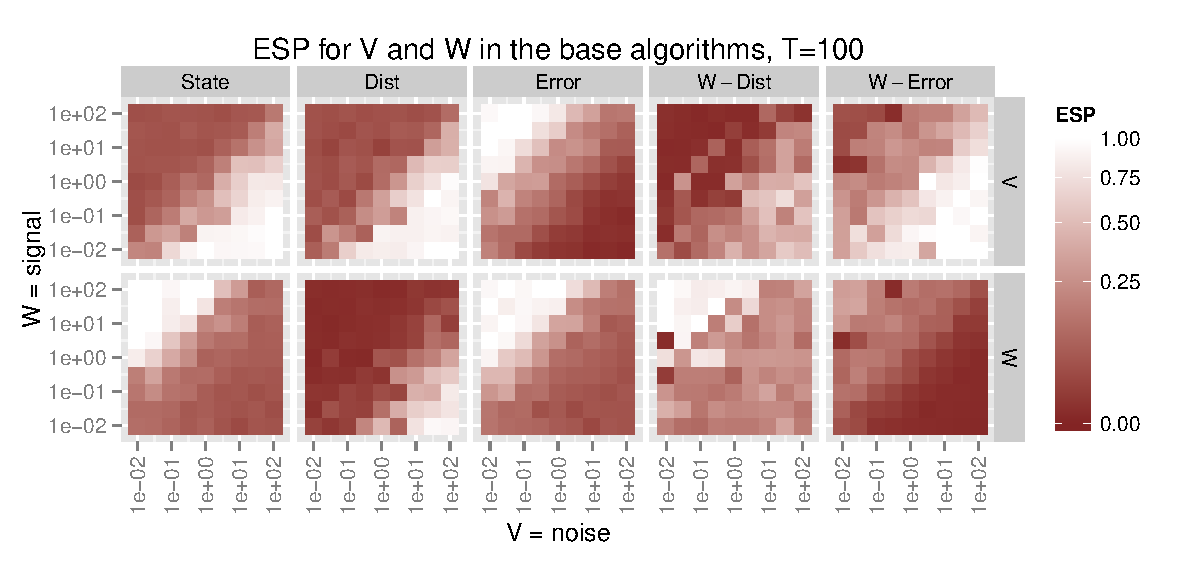
\includegraphics[width=0.7\textwidth]{plots/baseESplot1}
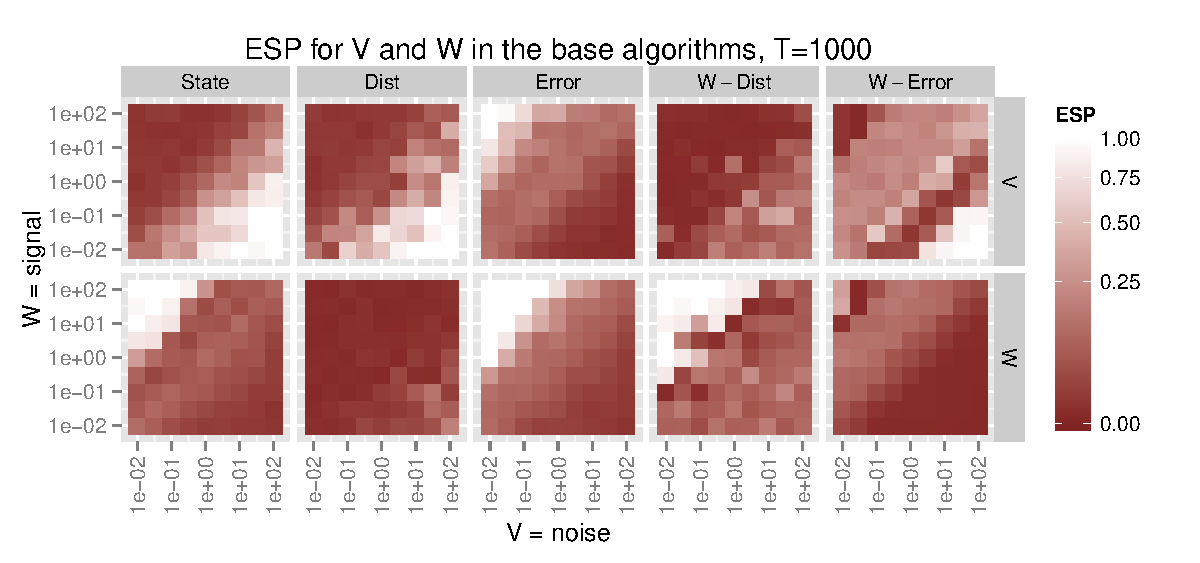
\includegraphics[width=0.7\textwidth]{plots/baseESplot2}
\caption{Effective sample proportion in the posterior sampler for a time series of lengths $T=100$ and $T=1000$, for $V$ and $W$, and for the state, scaled disturbance, scaled error, wrongly scaled disturbance, and wrongly scaled error samplers. $X$ and $Y$ axes indicate the true values of $V$ and $W$ respectively for the simulated data. Note that the signal-to-noise ratio is constant moving up any diagonal. In the upper left the signal is high, in the lower right the noise is high. Note that for plotting purposes, effective sample proportions larger than $1$ were rounded down to $1$.}
\label{baseESplot}
\end{figure}

\begin{figure}[!ht]
\centering
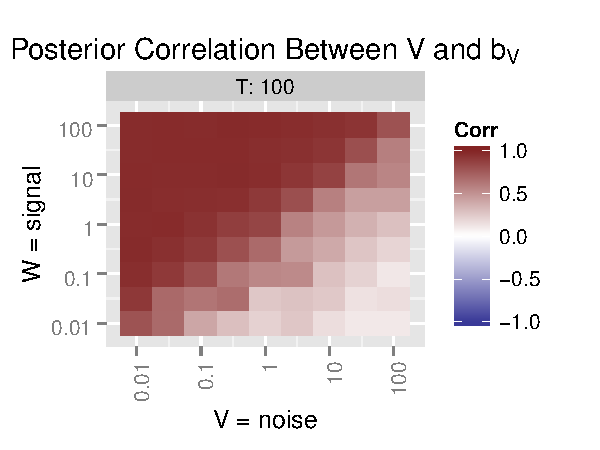
\includegraphics[width=0.24\textwidth]{plots/corplot1}
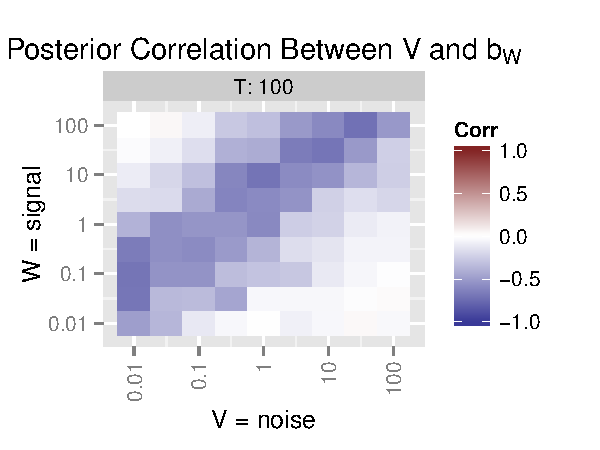
\includegraphics[width=0.24\textwidth]{plots/corplot2}
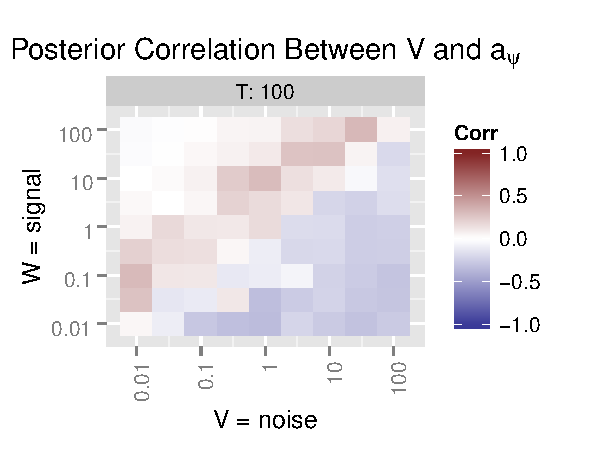
\includegraphics[width=0.24\textwidth]{plots/corplot3}
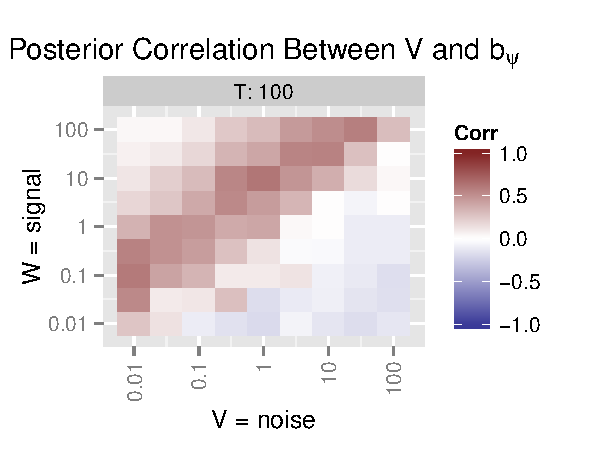
\includegraphics[width=0.24\textwidth]{plots/corplot4}
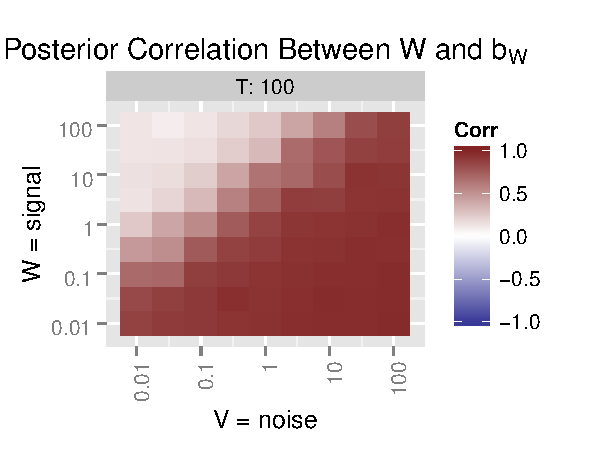
\includegraphics[width=0.24\textwidth]{plots/corplot5}
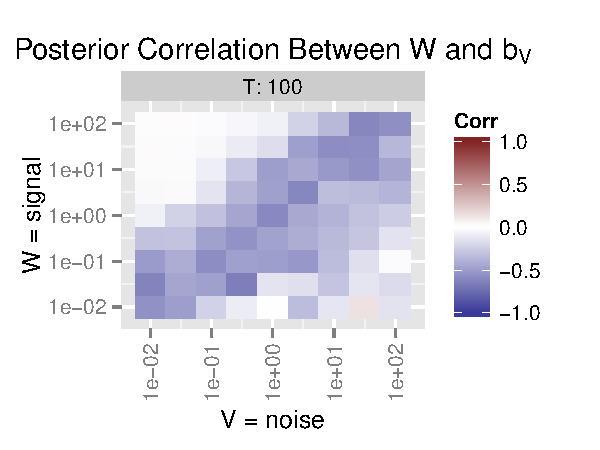
\includegraphics[width=0.24\textwidth]{plots/corplot6}
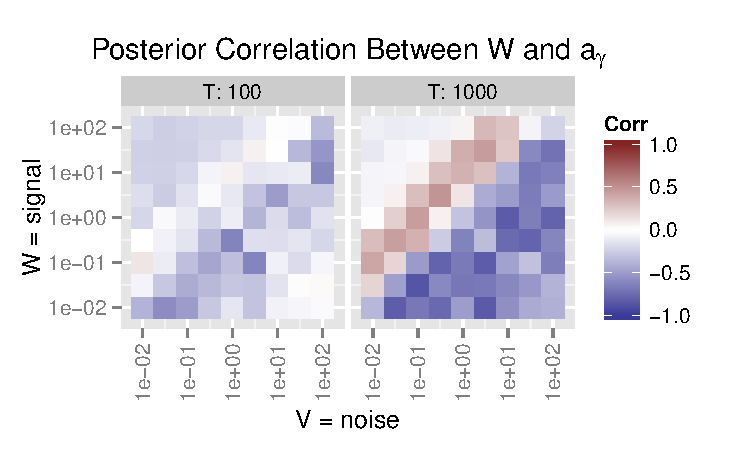
\includegraphics[width=0.24\textwidth]{plots/corplot7}
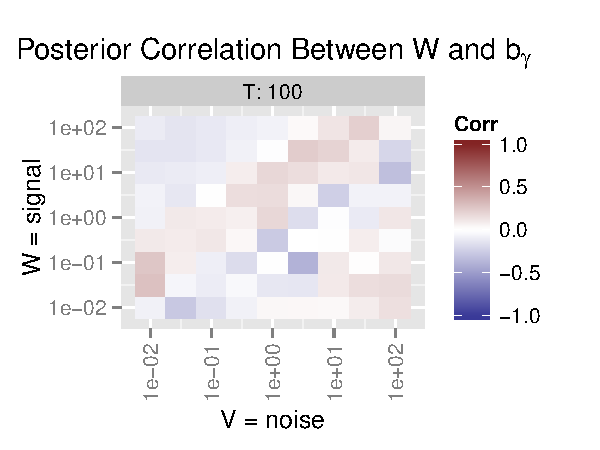
\includegraphics[width=0.24\textwidth]{plots/corplot8}
\caption{Posterior correlation between $V$ or $W$ and $b_V$ or $b_W$. $X$ and $Y$ axes indicate the true values of $V$ and $W$ respectively for the simulated data. Note that the signal-to-noise ratio is constant moving up any diagonal. In the upper left the signal is high, in the lower right the noise is high.}
\label{corplot}
\end{figure}

\subsection{GIS and CIS Results}

Based on the intuition in Section \ref{sec:DLMest} above, both the GIS and alternating algorithms should work best when at least one of the underlying base algorithms has a high ESP --- the basic idea is that when least one of the underlying algorithms has low serial dependence in the chain, the we should have low serial dependence in the GIS and alternating algorithms since the serial dependence in the bad DA algorithm is broken by adding a lower dependence step before the next iteration. This suggests that the Dist-Error GIS and alternating algorithms will have the best performance of the GIS and alternating algorithms using two DAs for both $V$ and $W$, especially for $R$ far away from one. When $R$ is near one it may offer no improvement however, especially for large $T$. The State-Dist algorithms should have trouble with $V$ when $R$ is high since both the state sampler and the scaled disturbance sampler have trouble with $V$ when $R$ is high. Similarly, the State-Error GIS algorithm should have trouble with $W$ when $R$ is low since both underlying samplers have trouble with $W$ when $R$ is low. Since the triple algorithms add the state sampler into the Dist-Error algorithms, it seems plausible that it might improve mixing for one of $V$ or $W$ since for $R$ different from one, the state sampler has good mixing for at least one of $V$ of $W$. 

There are a couple of ways to gain some intuition about what we expect the Full CIS algorithm to do before seeing the results. First, we mentioned in Section \ref{sec:DLMinter} that the Full CIS and the Dist-Error GIS algorithm consist of the same steps, just rearranged. This suggests that they should perform similarly so that we expect the Full CIS algorithm to have good mixing for both $V$ and $W$ when $R$ is sufficiently different from one. We can draw the same conclusion in a different way by noticing that in the Gibbs step for $V$, the CIS algorithm interweaves between the states and the scaled errors and in the Gibbs step for $W$ it interweaves between the states and the scaled disturbances. Since the state sampler has a high ESP for $V$ when $R<1$ and the scaled disturbance sampler has a high ESP for $V$ when $R>1$ we should expect the Full CIS sampler to have a high ESP for $V$ when $R$ is different from one. Similarly, since the state sampler has a high ESP for $W$ when $R>1$ and the scaled error sampler has a high ESP for $W$ when $R<1$, we should expect the Full CIS sampler to have a high ESP for $W$ when $R$ is different from one.

\begin{figure}[!ht]
\centering
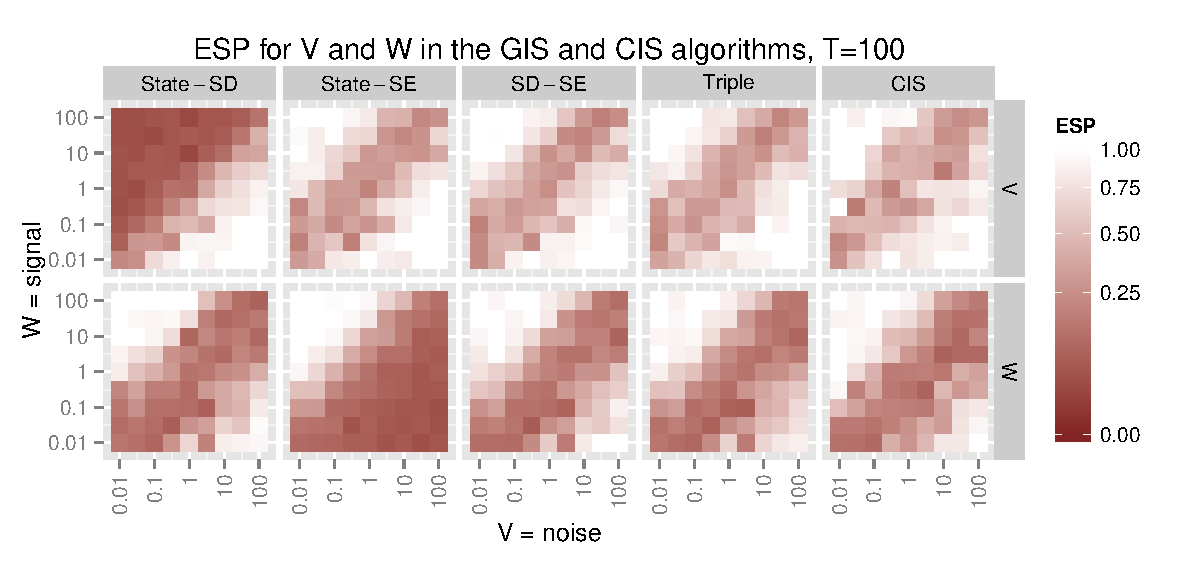
\includegraphics[width=0.7\textwidth]{plots/intESplot1}
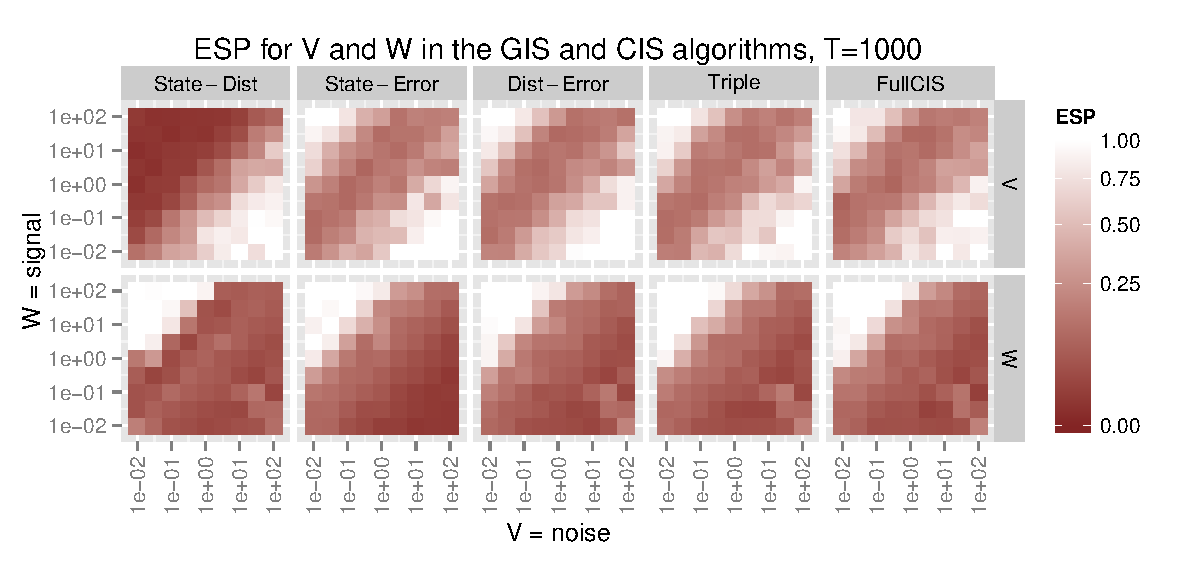
\includegraphics[width=0.7\textwidth]{plots/intESplot2}
\caption{Effective sample proportion in the posterior sampler for $V$ and $W$ in for $T=100$ and $T=1000$, in all three GIS samplers based on any two of the base samplers and the full CIS sampler. Horizontal and vertical axes indicate the true values of $V$ and $W$ respectively for the simulated data. Note that the signal-to-noise ratio is constant moving up any diagonal. In the upper left the signal is high, in the lower right the noise is high. Note that for plotting purposes, effective sample proportions larger than one were rounded down to one.}
\label{intESplot}
\end{figure}


We can verify most of these intuitions in Figure \ref{baseESplot}. First, the State-Dist GIS algorithm has high ESP for $W$ except for a narrow band where $R$ is near one, though this band becomes much wider as $T$ increases. The State-Dist GIS algorithm's mixing behavior for $V$ appears identical to the original state sampler --- high ESP when $R < 1$ and poor ESP when $R > 1$, and again the good region shrinks as $T$ increases. So this algorithm behaves as expected --- it takes advantage of the fact that the state and scaled disturbance DA algorithms make up a ``beauty and the beast'' pair for $W$ and thus improves mixing for $W$. However, the two underlying DA algorithms behave essentially identically for $V$ so there is no improvement. Similarly the State-Error GIS algorithm's ESP for $W$ is essentially identical to the state and scaled error algorithms' ESP for $W$ --- high when $R$ large and low when $R$ small.  For $V$, the State-Error algorithm has a high ESP when $R$ is far enough away from one, especially when $T$ is small. The Dist-Error GIS algorithm also behaves as predicted --- when $R$ is not too close to one it has high ESP for both $V$ and $W$, though as $T$ increases $R$ has too be farther away from one in order for the ESPs to be high and it has extra trouble with $W$ when $R$ is less than one but not small enough. The Dist-Error GIS algorithm behaves apparently identically to the Full CIS and triple GIS algorithms, with some differences when $T$ is small. The first of these is not surprising --- based on the intuition that the Dist-Error GIS and Full CIS algorithms are the same up to a reordering of each of their steps, we expected little if any difference. However, we had some hope that the triple GIS algorithm would improve upon the Dist-Error GIS algorithm somewhat by further breaking the correlation between iterations in the Markov chain. This did not happen and furthermore the State-Dist and State-Error samplers did not improve the ESP for $V$ or $W$ respectively over the original state sampler. When the underlying DA algorithms form a ``beauty and the beast'' pair, the interweaving algorithm appears to mix just as well as the best mixing single DA algorithm. Figure \ref{altESplot} allows us to see the ESP of the alternating algorithms in order to compare them to the GIS algorithms. There appears to be little practical difference between the alternating and interweaving versions of a given algorithm based on any two or three of the base DAs --- both take advantage of the beauty and the beast nature of their underlying DAs but dependence between the two DAs prevent the GIS version from improving on the alternating version. All of these results are summarized in Table \ref{tab:stnmix2} without distinguishing between the interweaving and alternating versions of an algorithm.

\begin{figure}[!ht]
\centering
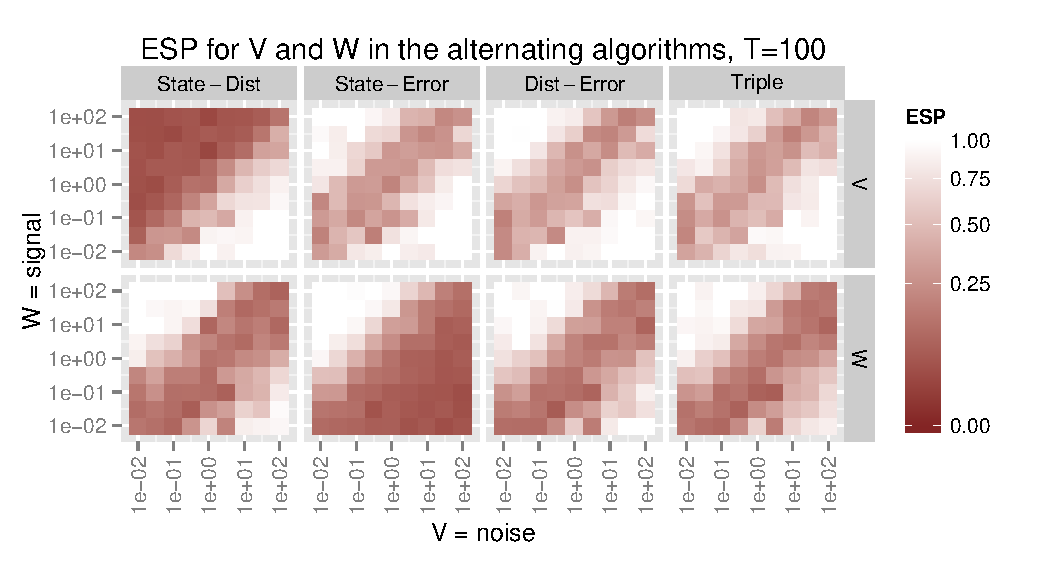
\includegraphics[width=0.7\textwidth]{plots/altESplot1}
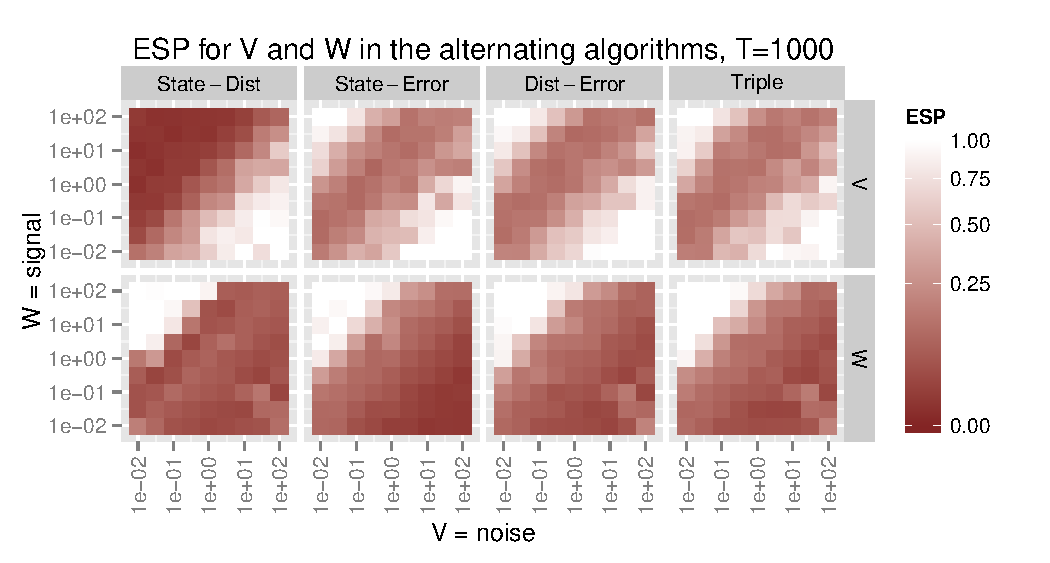
\includegraphics[width=0.7\textwidth]{plots/altESplot2}
\caption{Effective sample proportion in the posterior sampler for $V$ and $W$ in for $T=100$ and $T=1000$, in all four alternating samplers. Horizontal and vertical axes indicate the true values of $V$ and $W$ respectively for the simulated data. Note that the signal-to-noise ratio is constant moving up any diagonal. In the upper left the signal is high, in the lower right the noise is high. Note that for plotting purposes, effective sample proportions larger than one were rounded down to one.}
\label{altESplot}
\end{figure}

\begin{table}
  \centering
  \begin{tabular}{|l|ccccc|}\hline
    Parameter & State-Dist        & State-Error       & Dist-Error        & Triple            & Full CIS \\\hline
    V         & $R < 1$           & $R \not\approx 1$ & $R \not\approx 1$ & $R \not\approx 1$ & $R \not\approx 1$ \\
    W         & $R \not\approx 1$ & $R > 1$           & $R \not\approx 1$ & $R \not\approx 1$ & $R \not\approx 1$\\\hline
  \end{tabular}
  \caption{Rule of thumb for when each interweaving or alternating algorithm has a high effective sample size for each variable as a function of the true signal-to-noise ratio, $R=W/V$.}
  \label{tab:stnmix2}
\end{table}


\subsection{Computational time}\label{sec:LLMtime}

A more important question than how well the chain mixes from a practical standpoint is the full computational time required to adequately characterize the posterior distribution. In order to investigate this, we compute the natural log of the average time in minutes required for each sampler to achieve an effective sample size of 1000 --- in other words the log time per 1000 effective draws. All simulations were performed on a university cluster at Iowa State University with 24 Intel Xeon X5675 3.07 GHz processors. While different systems will yield different absolute times, the relative times should at least be similar. Figure \ref{baseinttimeplot} contains plots of the log time per 1000 effective draws for both $V$ and $W$ and for each of the base and interweaving samplers --- note that the scales change as $T$ changes. 

For $T=100$ and $T=1000$ we see that the pattern we saw for ESP begins also appears for time per 1000 effective draws. The state sampler becomes slow to reach 1000 effective draws for $V$ when $R>1$ and for $W$ when $R<1$. The scaled disturbance and scaled error samplers behave as expected --- the scaled disturbance sampler is slow for both $V$ and $W$ when $R>1$ while the scaled disturbance sampler is slow for both $V$ and $W$ when $R<1$. The Dist-Error GIS, Triple GIS and Full CIS algorithms appear to be the big winners here and are almost indistinguishable. All three algorithms are slightly slower for $V$ when $R$ is near one, and when $R$ is near or below one all three are slow for $W$. Compared to the state sampler though, all three offer large gains over most of the parameter space. When we compare the GIS algorithms to their alternating counterparts in terms of log time per 1000 effective draws, again there is little difference. Figure \ref{altinttimeplot} shows the log time per 1000 effective draws for the alternating algorithms and we see essentially the same pattern as we saw for the GIS algorithms with no clear advantage to the alternating or interweaving version of any algorithm.


\begin{figure}[!ht]
\centering
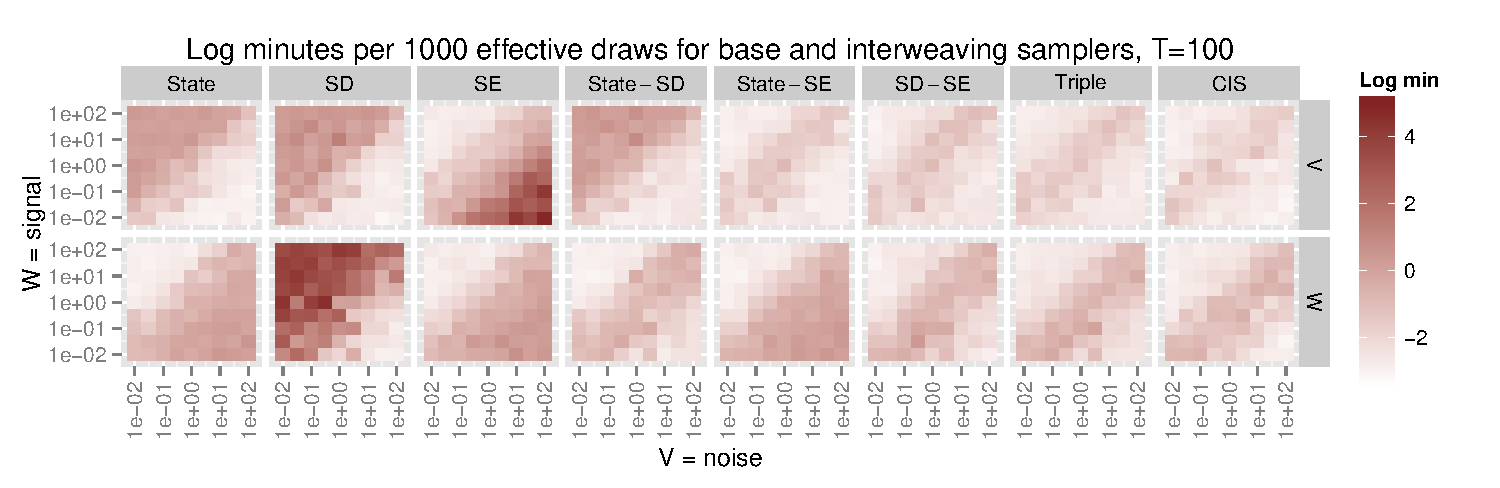
\includegraphics[width=0.8\textwidth]{plots/baseinttimeplot1}
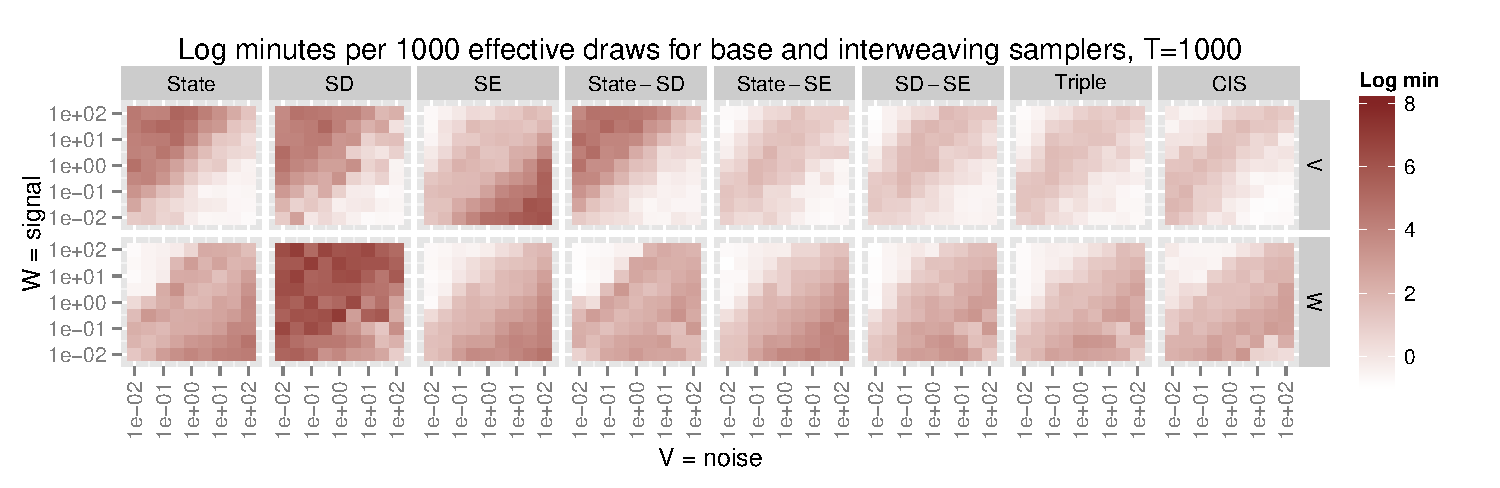
\includegraphics[width=0.8\textwidth]{plots/baseinttimeplot2}
\caption{Log of the time in minutes per 1000 effective draws in the posterior sampler for $V$ and $W$, for $T=100$ and $T=1000$, in the state, scaled disturbance and scaled error samplers and for all five interweaving samplers. Horizontal and vertical axes indicate the true values of $V$ and $W$ respectively for the simulated data. The signal-to-noise ratio is constant moving up any diagonal. In the upper left the signal is high, in the lower right the noise is high.}
\label{baseinttimeplot}
\end{figure}


\begin{figure}[!ht]
\centering
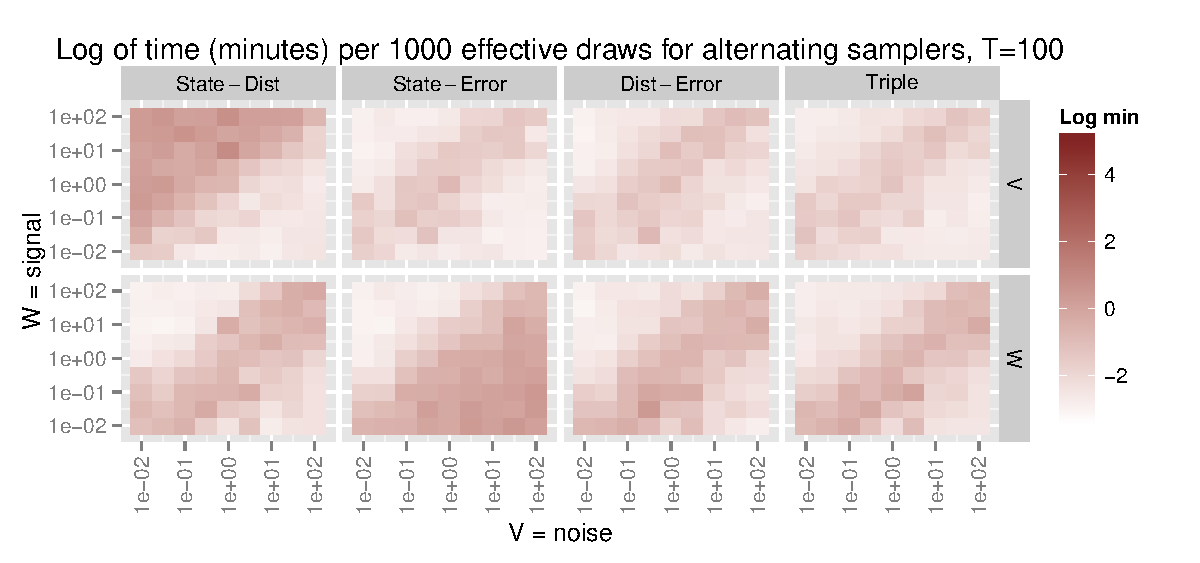
\includegraphics[width=0.49\textwidth]{plots/altinttimeplot1}
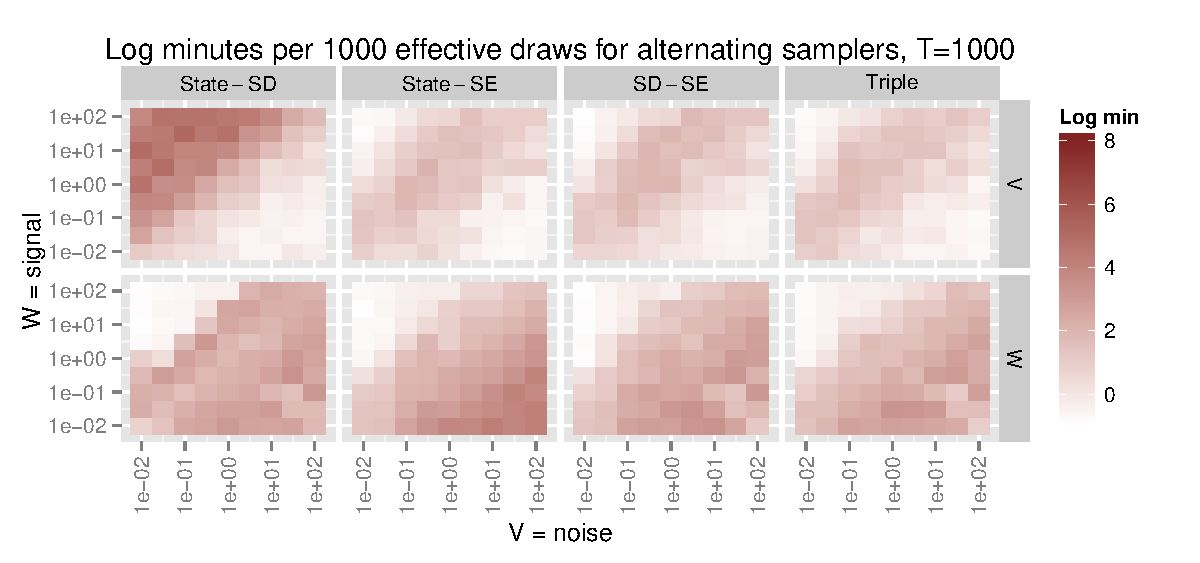
\includegraphics[width=0.49\textwidth]{plots/altinttimeplot2}
\caption{Log of the time in minutes per 1000 effective draws in the posterior sampler for $V$ and $W$, for $T=100$ and $T=1000$, in the alternating, GIS, and random kernel samplers. Horizontal and vertical axes indicate the true values of $V$ and $W$ respectively for the simulated data. The signal-to-noise ratio is constant moving up any diagonal. In the upper left the signal is high, in the lower right the noise is high.}
\label{altinttimeplot}
\end{figure}


\section{Discussion}\label{sec:Discussion}
Our results on computational time in Section \ref{sec:LLMtime} should be taken with a grain of salt because we did not put much effort into efficiently sampling from $p(W|V,\gamma_{0:T},y_{1:T}$ or $p(V|W,\psi_{0:T},y_{1:T})$. Both densities have the form
\[
p(x)\propto x^{-\alpha-1}\exp\left[-ax + b\sqrt{x} - \frac{\beta}{x}\right]
\]
where $\alpha,\beta,a>0$. This density is the same as the generalized inverse Gaussian distribution (see e.g. \citet{jorgensen1982statistical} for its properties; \citet{dagpunar1989easily} and \citet{devroye2012random} for generating random draws) when $b=0$, this is almost surely not the case in our application. It is possible that sampling from this density can be significantly improved in which case, the relative speed of the algorithms based on either the scaled errors or the scaled disturbances will improve significantly. On the other hand, it might be worth putting effort into drawing $V$ and $W$ jointly conditional on the scaled disturbances or the scaled errors. The conditional distribution of $V$ given $W$, $p(V|W,\gamma_{0:T},y_{1:T})$, is inverse gamma in our example and inverse Wishart in general, so it is easy to derive the marginal density $p(W|\gamma_{0:T},y_{1:T})$. In our local level model example, this density turns out to be very difficult to sample from and, in particular, is not easily approximated by a Gaussian distribution for rejection sampling or for a Metropolis step. 

We initially chose inverse Wishart priors for $V$ and $W$ partially because they are standard and partially for computational convenience. There are well known problems with this prior in the hierarchical model literature, e.g. \citet{gelman2006prior}, though less is known about the time series case. Given that the prior has potential problems and is inconvenient for the scaled disturbances and the scaled errors, a better choice of prior is probably out there. In particular, the conditionally conjugate prior for $\sqrt{W}$ using the scaled disturbances as the DA is a Gaussian distribution --- strictly speaking this prior is on $\pm \sqrt{W}$. If we use this prior for $\pm\sqrt{V}$ as well, the $V$ step in the Gibbs sampler becomes a draw from the generalized inverse Gaussian distribution. This prior has been used by \citet{fruhwirth2011bayesian} and \citet{fruhwirth2008bayesian} to speed up computation while using the scaled disturbances in hierarchical models and by \citet{fruhwirth2010stochastic} for time series models with a DA similar to the scaled disturbances (the latent states are scaled, but not centered). This prior seems particularly useful for variable selection problems, as evidenced by the papers which use it. We omit the results here, but using this prior does not alter our mixing results --- effective sample sizes were basically the same with either prior. There is a trade-off in computation time to consider, however. For example when using the scaled disturbances, the draw of $W|V,\gamma_{0:T},y_{1:T}$ is sped up by using the Gaussian prior on $\pm\sqrt{W}$ since it becomes a Gaussian draw while the $V|W,\gamma_{0:T},y_{1:T}$ is slower since it becomes a generalized inverse Gaussian draw instead of an inverse gamma. The gains outweigh the costs at least until a better way of sampling from $W$'s full conditional from the inverse gamma case is invented, but this only applies when $V$ is a scalar. When $V$ is a matrix, its full conditional becomes the matrix analogue of the generalized inverse Gaussian distribution and it is not clear how efficiently this density can be sampled from.

In our simulations with the original inverse gamma priors and the with the normal prior on the standard deviations we mentioned above, we varied the prior so that the prior mean was the true value of the parameters used to simulate the datasets. This may seem suspect at first glance, but there is a method to our madness. In the data augmentation for multilevel models literature, a key quantity is called the fraction of missing information (\citet{van2001art}, for example). When $\phi$ is the model parameter, $\theta$ is the data augmentation and $y$ is the data, the Bayesian fraction of missing information is defined as
\begin{align*}
  \mathcal{F}_B = I - [var(\phi|y)]^{-1}E[var(\phi|\theta,y)|y]
\end{align*}
while the EM fraction of missing information is defined as
\begin{align*}
  \mathcal{F}_{EM} = I - I_{obs}I_{aug}^{-1}
\end{align*}
where 
\begin{align*}
  I_{aug}=& \left.\mathrm{E} \left[-\left.\frac{\partial^2 \log p(\phi|\theta,y)}{\partial \phi \dot \partial \phi}\right| y,\phi\right]\right|_{\phi=\phi^*}\\
  \intertext{is the expected augmented Fisher information matrix and}
  I_{obs} =& -\left.\frac{\partial^2\log p(\phi|y)}{\partial\phi \dot \partial\phi}\right|_{\phi=\phi^*}
\end{align*}
is the observed Fisher information matrix while $\phi^*$ is the posterior mode. The rate of convergence of the EM algorithm is governed by $\mathcal{F}_{EM}$ while the maximum lag-1 autocorrelation in the Gibbs sampler for any linear function of the model parameters is governed by $\mathcal{F}_{B}$ --- the larger the spectral radius of $\mathcal{F}$, the high the autocorrelation. While $\mathcal{F}_{B}$ is difficult to compute, $\mathcal{F}_{EM}$ is often easier and is a decent approximation to $\mathcal{F}_{B}$ to the degree that the posterior distribution is Gaussian. We currently cannot analytically compute either of these quantities in our model, but the significance of the signal-to-noise ratio in our results is likely related. In particular, the EM fraction of missing information requires the expected and observed information matrices at the posterior mode. So the behavior of the samplers likely depends on the posterior model signal-to-noise ratio, or perhaps the ratio of the posterior model signal to the posterior mode ratio (depending on whether we take the mode of $R$, of $V$ and $W$ separately or of $V$ and $W$ together). Given the way we choose our priors, the posterior mode of $(V,W)$ is likely to be close to the true values of $V$ and $W$ used to simulate the data, especially for longer time series. If we used the same prior for each simulation, the posterior mode and the true values of $V$ and $W$ are less likely to be close for some true values of $V$ and $W$. In fact, in simulations with a constant prior (details not reported here), plots such as Figure \ref{baseESplot} look somewhat similar but with a much less stark difference in ESP over different regions of the parameter space.

Some previous work has been done in choosing data augmentations for time series models. In the AR(1) plus noise model, \citet{pitt1999analytic} find that the signal to noise ratio along with the AR(1) coefficient determine the convergence rate of a Gibbs sampler. In addition, they find that as the length of the time series increases, the convergence rate slows down and compute asymptotic convergence rates for an infinite time series. Both of these results are consistent with our findings and further suggest that the signal-to-noise ratio will play a key role in the fraction of missing information, Bayesian or EM, however, \citet{pitt1999analytic} assume that both of the variances are fixed for simplicity. In a continuous time model, \citet{roberts2004bayesian} find that the Gibbs sampler based on a NCP is at least as efficient as the Gibbs sampler based on the CP and sometimes it is much more efficient, depending on the true values of the parameters. It is unclear whether the time series dependence or something unique to the model is driving this, but it is interesting that the NCP is essentially always better. The dynamic regression model with a stationary AR(1) process on the regression coefficient has been studied in \citet{fruhwirth2004efficient}. They use both the states and the scaled disturbances and several other DAs motivated by some results for Gibbs samplers in the hierarchical model literature. When they examine the behavior of the resulting DA algorithms, \citet{fruhwirth2004efficient} find that the relative behavior of the scaled disturbance (in their language, the ``noncentered disturbances'') and state samplers are similar to our own results in the local level model, though now the signal-to-noise ratio is no longer the crucial quantity, but rather some function of it that also depends on the distribution of the covariate and the autocorrelation parameter in some currently unknown way. \citet{fruhwirth2004efficient} also find that none of the other DA algorithms they consider are more efficient than both the state sampler and the scaled disturbance sampler --- one of these always ends up being faster. This holds true both when they assume that the autorcorrelation parameter is known but when it is assumed unknown. This is encouraging since the extra complexity from adding a new parameter to the model (in our general DLM notation, this is in the form of $G_t$ depending on an additional unknown parameter) could drastically change the properties of the DA algorithms based on an AA (e.g. the scaled disturbances), but it appears the differences are relatively small.

\section{Appendix}\label{sec:append}

\subsection{Efficiently drawing from $p(W|V,\gamma,y)$ and $p(V|W,\psi,y)$}
Both of these two densities are of the form
\begin{align*}
\log p(x) = lp(x) & -ax + b\sqrt{x} - (\alpha + 1)\log x -\beta/x + C 
\end{align*}
for $x>0$ where $C$ is some constant, $\alpha$ and $\beta$ are the hyperparameters for $x$, and $a>0$ and $b\in \Re$ are parameters that depend on the data, $y$, the relevant data augmentation ($\psi$ or $\gamma$), and the other variable ($W$ or $V$). This density is not a known form and is difficult to sample from. We provide two different rejection sampling strategies below that work well under different circumstances, and combine them into a single strategy.

\subsubsection{Adaptive rejection sampling}
One nice strategy is to use adaptive rejection sampling, e.g. \citet{gilks1992adaptive}. This requires $lp(x)$ to be concave, which is easy enough to check. The second derivative of $lp(x)$ is:
\begin{align*}
\frac{\partial^2 lp(x)}{\partial x^2} &= -\frac{1}{4}bx^{-3/2} +(\alpha + 1)x^{-2} -2 \beta x^{-3}.
\end{align*}
Then we have
\begin{align*}
  &\frac{\partial^2 lp(x)}{\partial x^2} < 0 \iff \\
  &-\frac{b}{4}x^{3/2} + (\alpha + 1)x - 2\beta < 0
\end{align*}
which would imply that $lp(x)$ is concave. We can maximize the left hand side of the last equation very easily. When $b\leq 0$ the max occurs at $x=\infty$ such that $LHS > 0$, but when $b > 0$:
\begin{align*}
  \frac{\partial LHS}{\partial x} &= -\frac{3}{8}bx^{1/2} + \alpha + 1 = 0\\
  \implies & x^{max} = \frac{(\alpha + 1)^2}{b^2}\frac{64}{9}.
\end{align*}
Then we have
\begin{align*}
  LHS \leq LHS|_{x=x^{max}} = \frac{(\alpha + 1)^3}{b^2}\frac{64}{27} - 2\beta
\end{align*}
so that
\begin{align*}
  LHS|_{x=x^{max}} < 0 &\iff  \frac{(\alpha + 1)^3}{b^2}\frac{64}{27} < 2\beta\\
    &\iff b > \left(\frac{(\alpha + 1)^3}{\beta}\right)^{1/2}\frac{4\sqrt{2}}{3\sqrt{3}}.
\end{align*}
This last condition is necessary and sufficient for $lp(x)$ to be globally (for $x>0$) concave since $b < 0$ forces $LHS > 0$ for some $x$. When the condition is satisfied, we can use adaptive rejection sampling --- which is already implemented in the \verb0R0 package \verb0ars0. We input the initial evalutions of $lp(x)$ at the mode $x^{mode}$ and at $2x^{mode}$ and $0.5x^{mode}$ in order to get the algorithm going.

\subsubsection{Rejection sampling on the log scale}
When $b \leq \left(\frac{(\alpha + 1)^3}{\beta}\right)^{1/2}\frac{4\sqrt{2}}{3\sqrt{3}}$, which happens often --- especially for small $T$ --- we need to rely on a different method to sample from $p(x)$. A naive approach would be to construct a normal or $t$ approximation to $p(x)$ and use that as a proposal in a rejection sampler. It turns out that this is often very inefficient, but for $y=log(x)$ the approach works well. Note that
\begin{align*}
  p_y(y) = p_x(e^y)e^y
\end{align*}
so that we can write the log density of $y$ as (dropping the subscripts):
\begin{align*}
  lp(y) = -ae^y + be^{y/2} - \alpha y - \beta e^{-y}.
\end{align*}
The mode of this density $y^{mode}$ can be easily found numerically, and the second derivative is:
\begin{align*}
  \frac{\partial^2 lp(y)}{\partial y^2} = -ae^y + \frac{b}{4}e^{y/2} - \beta e^{-y}.
\end{align*}
The $t$ approximation then uses the proposal distribution 
\begin{align*}
  t_{v}\left(y^{mode}, \left[\left.\frac{\partial^2 lp(y)}{\partial y^2}\right|_{y=y^{mode}}\right]^{-1}\right).
\end{align*}
In practice choosing degrees of freedom $v=1$ works very well over the region of the parameter space where adaptive rejection sampling cannot be used. We can easily use this method when adaptive rejection sampling does not work, then transform $y$ back to $x$. It remains to check that the tails of $t$ distribution dominate the tails of our target distribution. Let $lq(y)$ denote the log density of the proposoal distribution. Then we need
\begin{align*}
  lp(y) - lq(y) \leq M\\
  \intertext{for some constant M, i.e.}
  -ae^y + be^{y/2} - \alpha y - \beta e^{-y} -\left(\frac{v+1}{2}\right)\log\left[1 + \frac{1}{v}\left(\frac{y-\mu}{\sigma}\right)\right]\leq M
\end{align*}
where $a>0$, $\alpha>0$, $\beta>0$, $v>0$, $\sigma>0$, and $b,\mu\in \Re$. We can rewrite the LHS as
\begin{align*}
    e^{y/2}(b-ae^{y/2}) - \alpha y - \beta e^{-y} -\left(\frac{v+1}{2}\right)\log\left[1 + \frac{1}{v}\left(\frac{y-\mu}{\sigma}\right)\right].
\end{align*}
So as $y\to\infty$ this quantity goes to $-\infty$ since the first term will eventually become negative no matter the value of $b$, and all other terms are always negative. Similarly as $y\to\-\infty$ this quantity goes to $-\infty$. Now pick any interval $(y_1,y_2)$ such that outside of the interval, $LHS<\epsilon$. Since treated as a function of $y$ the LHS is clearly continuous, it attains a maximum on this interval, and thus is bounded.

\subsubsection{Intelligently choosing a rejection sampler}
In practice, adaptive rejection sampling is relatively efficient for $p_x(x)$ but inefficient for $p_y(y)$ --- so much so that rejection sampling with the $t$ approximation for $p_y(y)$ is more efficient. To minimize computation time, it is best to use adaptive rejection sampling for $p_x(x)$ when the concavity condition is satisfied. When it is not, the $t$ approximation works well enough.

\subsection{Efficiently drawing from $p(W|V,\tilde{\gamma},y)$ and $p(V|W,\tilde{\psi},y)$ in the LLM}

Both the density of $\log(W)|V,\tilde{\gamma}_{0:T},y_{1:T}$ and the density of $\log(V)|W,\tilde{\psi}_{0:T},y_{1:T}$ have the following form:
\begin{align*}
  p(y)\propto \exp\left[-\alpha y - ae^{-y} + be^{-y/2} - ce^y\right].
\end{align*}
where $\alpha>0$, $a>0$, $c>0$, and $b\in \Re$. The log density is:
\begin{align*}
  lp(y) = -\alpha y - ae^{-y} + be^{-y/2} - ce^y + C
\end{align*}
where $C$ is some constant. We only provide one strategy for rejection sampling from this density: the $t$ approximation. Similar reasoning to above shows that we can use a $t$ distribution as a proposal in a rejection sampler. Now we choose the location parameter by maximizing $lp(y)$ in $y$ numerically to find the mode, $y^{mode}$. Next the second derivative of $lp(y)$ is given by
\begin{align*}
  \frac{\partial^2 lp(y)}{\partial y^2} = -ae^{-y} + \frac{b}{4}e^{-y/2}-ce^y.
\end{align*}
We then set the scale parameter to be
\begin{align*}
  -\left[\left.\frac{\partial^2 lp(y)}{\partial y^2}\right|_{y=y^{mode}}\right]^{-1}
\end{align*}
as in the normal approximation, and the degrees of freedom parameter to $v=1$. This rejection sampler is tolerably efficient for our purposes, but it is not fast.




\clearpage

\bibliographystyle{plainnat}
\bibliography{dlmasis}
\end{document}




